% This work is licensed under the Creative Commons
% Attribution-NonCommercial-ShareAlike 4.0 International License. To view a copy
% of this license, visit http://creativecommons.org/licenses/by-nc-sa/4.0/ or
% send a letter to Creative Commons, PO Box 1866, Mountain View, CA 94042, USA.

% (c) Eric Kunze, 2020

%%%%%%%%%%%%%%%%%%%%%%%%%%%%%%%%%%%%%%%%%%%%%%%%%%%%%%%%%%%%%%%%%%%%%%%%%%%%%%%
% Template for lecture notes and exercises at TU Dresden.
%%%%%%%%%%%%%%%%%%%%%%%%%%%%%%%%%%%%%%%%%%%%%%%%%%%%%%%%%%%%%%%%%%%%%%%%%%%%%%%

\documentclass[ngerman, a4paper, 11pt]{article}

\usepackage[top=2.5cm,bottom=2.5cm,left=2.5cm,right=2.5cm]{geometry}
% \usepackage[left=2.1cm,right=3.1cm,bottom=3cm,footskip=0.75cm,headsep=0.5cm]{geometry}

\usepackage[ngerman]{babel}
\usepackage[utf8]{inputenc}

\usepackage{parskip}  	% split paragraphs by vspace instead of intendations
\usepackage[onehalfspacing]{setspace} % increase row-space

\usepackage{lmodern}
\usepackage{eufrak}
\usepackage{ulem} 		% better underlines
\usepackage[autostyle=true,english=british]{csquotes}

\usepackage[scale=0.95]{opensans}	% new font OpenSans
%\newcommand*{\fosfamily}{\fontfamily{fos}\selectfont}
\DeclareTextFontCommand{\textos}{\fosfamily}

\usepackage{xifthen}


%%%%%%%%%%%%%%%%%%%%%%%%%%%%%%%%%%%%%%%%%%%%%%%%%%%%%%%%%%%%%%%%%%%%%%%%%%%%%%%%%%%%%%%%%%%%%%%%%%%%%%%

\newcommand{\name}{Eric Kunze}
\newcommand{\matnr}{4679202}
\newcommand{\email}{\href{mailto:eric.kunze@mailbox.tu-dresden.de}{\ttfamily eric.kunze@mailbox.tu-dresden.de}}

\newcommand{\modul}{Funktionentheorie}
\newcommand{\semester}{Sommersemester 2020}

%\renewcommand{\tutor}{Dr. Legrand}
%\renewcommand{\gruppe}{Tag x. DS, (un)gerade Woche}

\newcommand{\professor}{Prof. Dr. Stefan Siegmund}
\newcommand{\fakultaet}{Mathematik}
\newcommand{\institut}{Analysis}
\newcommand{\lehrstuhl}{Dynamik und Steuerung}

%%%%%%%%%%%%%%%%%%%%%%%%%%%%%%%%%%%%%%%%%%%%%%%%%%%%%%%%%%%%%%%%%%%%%%%%%%%%%%%%%%%

\usepackage[smallequationskip]{../../texmf/tex/latex/mathworkMathTUD}
\usepackage{../../texmf/tex/latex/mathoperatorsMathTUD}

%%%%%%%%%%%%%%%%%%%%%%%%%%%%%%%%%%%%%%%%%%%%%%%%%%%%%%%%%%%%%%%%%%%%%%%%%%%%%%%%%%%
% graphics

\usepackage{xcolor}
\usepackage[table,dvipsnames]{tudscrcolor}
\usepackage{graphicx}
\usepackage{tcolorbox}

\usepackage[font=small,labelfont=bf]{caption} % captions of non-floated figures

\usepackage{pgf}
\usepackage{pgfplots}
\pgfplotsset{compat=1.10}   % in my packages used compat=1.15
\usepgfplotslibrary{fillbetween}

\usepackage{tikz}
\usetikzlibrary{patterns,arrows,calc,decorations.pathmorphing,backgrounds, positioning,fit,petri,decorations.fractals}
\usetikzlibrary{matrix}


%%%%%%%%%%%%%%%%%%%%%%%%%%%%%%%%%%%%%%%%%%%%%%%%%%%%%%%%%%%%%%%%%%%
% tabulars

\usepackage{tabularx} 
\usepackage{multirow}



%%%%%%%%%%%%%%%%%%%%%%%%%%%%%%%%%%%%%%%%%%%%%%%%%%%%%%%%%%%%%%%%%%%%%%%%%%%%%%%%%%%%%%%%%%%%%%%%%%%%%%%

%%%%%%%%%%%%%%%%%%%%%%%%%%%%%%%%%%%%%%%%%%%%%%%%%%%%%%%%%%%%%%%%%%%
%                             COUNTER                             %
%%%%%%%%%%%%%%%%%%%%%%%%%%%%%%%%%%%%%%%%%%%%%%%%%%%%%%%%%%%%%%%%%%%
\usepackage{chngcntr}

% automatic reset of section after chapter ended 
\pretocmd{\chapter}{\setcounter{section}{0}}{}{}

% automatic reset of equation counter in each section
\pretocmd{\section}{\setcounter{equation}{0}}{}{}


\usepackage{chngcntr}
\newcounter{taskcount}
\newcounter{blattcount}
\newcounter{themcount}

\numberwithin{page}{blattcount}

\counterwithout{equation}{section}
\counterwithin{equation}{blattcount}
\counterwithin{figure}{blattcount}
\counterwithin{table}{blattcount}

%\counterwithin{themcount}{chapter}
%\numberwithin{page}{blattcount}
\counterwithin{taskcount}{blattcount}

%%%%%%%%%%%%%%%%%%%%%%%%%%%%%%%%%%%%%%%%%%%%%%%%%%%%%%%%%%%%%%%%%%%%%%%%%%%%%%%%%%%%%%%%%%%%%%%%%%%%%%%

%%%%%%%%%%%%%%%%%%%%%%%%%%%%%%%%%%%%%%%%%%%%%%%%%
% Environment for a new exercise sheet
\usepackage{tcolorbox}
\newcommand{\header}{%
        {\fosfamily%
            \fcolorbox{cddarkblue}{cdblue!20}{%
                \begin{minipage}{\dimexpr0.7\linewidth-\fboxrule-\fboxsep}
                    {\huge \textbf{Hausaufgaben}} \vspace{3pt} \\
                    \textbf{\modul} -- Übungsblatt \theblattcount
                \end{minipage}%
                \begin{minipage}{\dimexpr0.3\linewidth-\fboxrule-\fboxsep}
                    \flushright \textbf{\name} \\
                    Matr.-Nr. \matnr
                \end{minipage}%
        }}%
    }%

\NewDocumentEnvironment{exercisePage}{O{}}{%
    \pagebreak%
    \stepcounter{blattcount} \setcounter{page}{1}%
    \header \\[6pt]
    \setcounter{figure}{0}
    \setcounter{equation}{0}%
    \setcounter{table}{0}%
    \setcounter{themcount}{0}
    %
    \ifthenelse{\isempty{#1}}{}{%
        {\fosfamily \itshape Thema: #1} \par%\\[12pt]%
    }
}{}

%%%%%%%%%%%%%%%%%%%%%%%%%%%%%%%%%%%%%%%%%%%%%%%%%
% Packages for theorem environments
\usepackage[ntheorem,framemethod=TikZ]{mdframed}
\usepackage{amsmath,amssymb,amsfonts,mathtools}
\usepackage[amsmath,thmmarks,framed]{ntheorem}

%%%%%%%%%%%%%%%%%%%%%%%%%%%%%%%%%%%%%%%%%%%%%%%%%
% theorem environments for exercises and solutions

\newcommand{\skiparound}{10pt}

% >> Exercises
\theoremstyle{plain}
\theoremheaderfont{\fosfamily\normalsize\bfseries\upshape}
\theorembodyfont{\normalsize}
\theoremseparator{.}
\theoremsymbol{}

\newmdtheoremenv[%
    backgroundcolor=cdblue!5,%
    linecolor=cddarkblue,%
    skipabove=\skiparound,%
    skipbelow=\skiparound,%
    nobreak,%
]{exercise}[taskcount]{Übung}

\newmdtheoremenv[%
    backgroundcolor=cdblue!5,%
    linecolor=cddarkblue,%
    skipabove=\skiparound,%
    skipbelow=\skiparound,%
    nobreak,%
]{homework}[taskcount]{Hausaufgabe}

\newmdtheoremenv[%
    backgroundcolor=cdblue!5,%
    linecolor=cddarkblue,%
    skipabove=\skiparound,%
    skipbelow=\skiparound,%
    nobreak,%
]{task}[taskcount]{Aufgabe}

%%%%%%%%%%%%%%%%%%%%%%%%%%%%%%%%%%%%%%%%%%%%
% >> Lemma
\theoremstyle{plain}
\theoremheaderfont{\fosfamily\normalsize\bfseries\upshape}
\theorembodyfont{\itshape}
\theoremseparator{.}
\theoremsymbol{\textleaf}
\theorempreskip{6pt}
\theorempostskip{6pt}
\newtheorem{lemma}{Lemma}
\counterwithin{lemma}{blattcount}

% >> Solution
\theoremstyle{nonumberplain}
\theoremheaderfont{\normalfont\normalsize\bfseries}
\theorembodyfont{\normalfont}
\theoremseparator{\textbf{.}}
\theorempreskip{5pt}
\theorempostskip{5pt}
\theoremsymbol{$\square$}
\newtheorem{solution}{Lösung}

% >> proof
\newtheoremstyle{proofstyle}%
{\item[\hskip\labelsep {\theorem@headerfont ##1}\theorem@separator]}%
{\item[\hskip\labelsep {\theorem@headerfont ##1}\ (##3)\theorem@separator]}

\theoremstyle{proofstyle}
\theoremheaderfont{\normalsize\slshape}
\theorembodyfont{}
\theoremseparator{.}
\theorempreskip{0pt}
\theorempostskip{5pt}
\theoremsymbol{$\square$}
\newtheorem{proof}{Beweis}

% >> Equivalences
\newcommand{\hinrichtung}{\item[\bfseries ($\boldsymbol{\Rightarrow}$)]}
\newcommand{\rueckrichtung}{\item[\bfseries ($\boldsymbol{\Leftarrow}$)]}

\newenvironment{equivalence}[1][]{%
    \ifthenelse{\isempty{#1}}%
        {\begin{description}}%
        {\begin{description}[topsep=-\parskip]}%
}{%
        \end{description}%
}%

% >> inductions
\newcommand{\ianfang}[1][]{%
    \ifthenelse{\isempty{#1}}{%
        % no parameter
        \item[\textbf{(IA)}]%
    }{%
        %parameter exists
        \item[\textbf{(IA)}] {#1 :} %\hfill \\%
    }%
}

\newcommand{\ivorraussetzung}{\item[\bfseries (IV)]}

\newcommand{\ischritt}[1][]{%
    \ifthenelse{\isempty{#1}}{%
        % no parameter
        \item[\textbf{(IS)}]
    }{%
        % parameter exists
        \item[\textbf{(IS)}] {#1 :} %\\
    }%
}

% two optional arg's:
% #1 = induced variable 
% #2 = vert. space before (IA): parskip (default) or nopreskip
\NewDocumentEnvironment{induction}{O{} O{}}{%
    \ifthenelse{ \isempty{#1} }{}{%
        Vollständige Induktion nach #1:
    }%---
    \ifthenelse{ \equal{#2}{nopreskip} }{%
        \begin{description}[topsep=-\parskip]
    }{%
        \begin{description}
    }%
}{%
    \end{description}%
}


%%%%%%%%%%%%%%%%%%%%%%%%%%%%%%%%%%%%%%%%%%%%%%%%%%%%%%%%%%%%%%%%%%%%%%%%%%%%%%%%%%%

%%%%%%%%%%%%%%%%%%%%%%%%%%%%%%%%%%%%%%%%%%%%%%%%%%%%%%%%%%%%%%%%%%%
%                           TITLEPAGE                             %
%%%%%%%%%%%%%%%%%%%%%%%%%%%%%%%%%%%%%%%%%%%%%%%%%%%%%%%%%%%%%%%%%%%

\newcommand{\makeTUtitle}[1][]{%
	\begin{titlepage}
		\pagecolor{cddarkblue!90} \color{white}%
		\raggedright \fosfamily%
		\setlength{\parindent}{0pt}% 
	% Logo / Kopf
		\hspace{-18.6mm} %
		
\includegraphics[scale=0.6]{TUD-white.pdf} \\
		\vspace{3mm} 
		\begin{tabular}{m{\textwidth}}
			\hline
			\hspace{-4pt}\small{\textbf{Fakultät \fakultaet} Institut für \institut, Professur für \lehrstuhl} \\
			\hline
		\end{tabular} \\
	% Titel
		\vspace{5cm}
		{\Huge\bfseries \MakeUppercase \modul \par}
		\ifthenelse{\isempty{#1}}{}{
			\vspace{0.5cm}%
			{\Large \itshape #1} \\%
		}
		\vspace{1.5cm}
		\textbf{{\Large \professor}} \par
		\vspace{0.5cm}
		{\large \semester}
	% Fußzeile
		\vfill%
		\begin{tabular}{lll}
			Autor  & : & \name \\
			E-Mail & : & \email \\
		\end{tabular}%
	\end{titlepage}
	\nopagecolor
}

%%%%%%%%%%%%%%%%%%%%%%%%%%%%%%%%%%%%%%%%%%%%%%%%%%%%%%%%%%%%%%%%%%%%%%%%%%%%%%%%%%%


%%%%%%%%%%%%%%%%%%%%%%%%%%%%%%%%%%%%%%%%%%%%%%%%%%%%%%%%%%%%%%%%%%%
%                          HIGHLIGHTING                           %
%%%%%%%%%%%%%%%%%%%%%%%%%%%%%%%%%%%%%%%%%%%%%%%%%%%%%%%%%%%%%%%%%%%
\newcommand{\begriff}[1]{\textbf{#1}}
\newcommand{\person}[1]{\textsc{#1}}

%%%%%%%%%%%%%%%%%%%%%%%%%%%%%%%%%%%%%%%%%%%%%%%%%%%%%%%%%%%%%%%%%%%
%                            EQUATIONS                            %
%%%%%%%%%%%%%%%%%%%%%%%%%%%%%%%%%%%%%%%%%%%%%%%%%%%%%%%%%%%%%%%%%%%

\setlength\abovedisplayshortskip{0pt plus 3pt}%
\setlength\belowdisplayshortskip{4pt plus 2pt minus 2pt}%
\setlength\abovedisplayskip{1pt plus 1pt minus 2pt}%
\setlength\belowdisplayskip{1pt plus 1pt minus 2pt}%


%%%%%%%%%%%%%%%%%%%%%%%%%%%%%%%%%%%%%%%%%%%%%%%%%%%%%%%%%%%%%%%%%%%
%                          ENUMERATIONS                           %
%%%%%%%%%%%%%%%%%%%%%%%%%%%%%%%%%%%%%%%%%%%%%%%%%%%%%%%%%%%%%%%%%%%
\usepackage{enumerate}
\usepackage[inline]{enumitem} 		%customize label

\renewcommand{\labelitemi}{\raisebox{1pt}{\scalebox{.6}{$\blacksquare$}}}
\renewcommand{\labelitemii}{$\vartriangleright$}
\renewcommand{\labelitemiii}{--}
% Variantionen des Dreiecks als Aufzählungszeichen $\blacktriangleright$ / $\vartriangleright$ / $\triangleright$

\renewcommand{\labelenumi}{(\alph{enumi})}
\renewcommand{\labelenumii}{\roman{enumii}.}
%\renewcommand{\labelenumiii}{\roman{enumiii}.}

%%%%%%%%%%%%%%%%%%%%%%%%%%%%%%%%%%%%%%%%%%%%%%%%%%%%%%%%%%%%%%%%%%%
%                            LISTINGS                             %
%%%%%%%%%%%%%%%%%%%%%%%%%%%%%%%%%%%%%%%%%%%%%%%%%%%%%%%%%%%%%%%%%%%
\usepackage{listings}

%%%%%%%%%%%%%%%%%%%%%%%%%%%%%%%%%%%%%%%%%%%%%%%%%%%%%%%%%%%%%%%%%%%%%%%%%%%%%%%%%%%%%%%%%%%%%%%%%%%%%%%
% references 

\usepackage[unicode,bookmarks=true]{hyperref}
\hypersetup{
	% pdfborder={0 0 0}			% no boxed around links
	pdfborderstyle={/S/U/W 1},	% underlining insteas of boxes
	linkbordercolor=cdblue,
	urlbordercolor=cdblue
	%	colorlinks,
	%	citecolor=black,
	%	filecolor=cddarkblue!80,
	%	linkcolor=black,
	%	urlcolor=cddarkblue!80
}


\usepackage{cleveref}
\crefname{lemma}{Lemma}{Lemmata}
\crefname{exercise}{Übung}{Übungen}
\crefname{homework}{Hausaufgabe}{Hausaufgaben}
\crefname{task}{Aufgabe}{Aufgaben}

%\crefformat{equation}{#2Gleichung~(#1)#3}

\usepackage{bookmark}		% pdf-bookmarks

%%%%%%%%%%%%%%%%%%%%%%%%%%%%%%%%%%%%%%%%%%%%%%%%%%%%%%%%%%%%%%%%%%%%%%%%%%%%%%%%%%%%%%%%%%%%%%%%%%%%%%%
%%%%%%%%%%%%%%%%%%%%%%%%%%%%%%%%%%%%%%%%%%%%%%%%%%%%%%%%%%%%%%%%%%%%%%%%%%%%%%%%%%%%%%%%%%%%%%%%%%%%%%%
%%%%%%%%%%%%%%%%%%%%%%%%%%%%%%%%%%%%%%%%%%%%%%%%%%%%%%%%%%%%%%%%%%%%%%%%%%%%%%%%%%%%%%%%%%%%%%%%%%%%%%%
%%%%%%%%%%%%%%%%%%%%%%%%%%%%%%%%%%%%%%%%%%%%%%%%%%%%%%%%%%%%%%%%%%%%%%%%%%%%%%%%%%%%%%%%%%%%%%%%%%%%%%%
%%%%%%%%%%%%%%%%%%%%%%%%%%%%%%%%%%%%%%%%%%%%%%%%%%%%%%%%%%%%%%%%%%%%%%%%%%%%%%%%%%%%%%%%%%%%%%%%%%%%%%%
%%%%%%%%%%%%%%%%%%%%%%%%%%%%%%%%%%%%%%%%%%%%%%%%%%%%%%%%%%%%%%%%%%%%%%%%%%%%%%%%%%%%%%%%%%%%%%%%%%%%%%%


%---------------------------------------
% additional packages
%---------------------------------------



%---------------------------------------
% additional comands
%---------------------------------------

\DeclareMathOperator{\Ln}{Ln}
\DeclareMathOperator{\Arg}{Arg}
\DeclareMathOperator{\im}{im}
%%%%%%%%%%%%%%%%%%%%%%%%%%%%%%%%%%%%%%%%%%%%%%%%%%%%%%%%%%%%%%%%%%%%%%%%%%%%%%%%%%%%%%%%%%%%%%%%%%%%%%%


\begin{document}

\makeTUtitle[Übungen]


\begin{exercisePage}[Komplexe Zahlen \& Differenzierbarkeit]
%
% Aufgabe 1.1
\begin{task} \label{task: 1.1}
	Wo liegen in der Gaußschen Zahlenebene diejenigen Punkte $z$, für die gilt
	\begin{enumerate}[leftmargin=*, nolistsep, topsep=-\parskip]
		\item $0 < \Re(\i z) < 2\pi$
		\item  $\abs{z - z_1} = \abs{z - z_2}$ ($z_1, z_2 \in \CC$ gegeben)
		\item $\abs{z} + \Re(z) < 1$
		\item $z^5 = 1$
		\item $z = 3 - \i + 5e^{\i t}$ ($0 \le t \le \pi$)
		\item $z = te^{\i t}$ ($t \ge 0$)
	\end{enumerate}
\end{task}

\begin{enumerate}[leftmargin=*, label=(zu \alph*)]
	\item Mit $z = a + b\i$ ist $\i*z = -b + a\i$, d.h. $\Re(\i * z) = - \Im(z)$.
	\item Der Term $\abs{z - z_1}$ beschreibt den Abstand zwischen $z$ und $z_1$, d.h.  $\abs{z - z_1} = \abs{z - z_2}$ beschreibt alle Punkte, die von $z_1$ und $z_2$ den gleichen Abstand haben. Dies sind alle Punkte, die auf der Geraden mit Normale $n = \quer{z_1z_2}$ liegen, d.h. $z$ erfülle die Bedingung $\scal{n}{\frac{1}{2} z_1 + \frac{1}{2} z_2 - z} = 0$, wobei $z, z_1, z_2$ als Punkte im $\R^2$ mit dem Standardskalarprodukt zu verstehen sind.
	\item Sei $z = a + b\i$, dann lässt sich die Gleichung schreiben als
	\begin{equation*}
		\begin{alignedat}{3}
			\sqrt{a^2 + b^2} + a &< 1 &\equivalent& &\sqrt{a^2 + b^2} &< 1 - a \\
			&&\equivalent& &a^2 + b^2 &< 1 - 2a + a^2 \\
			&&\equivalent& &y^2 &< 1 - 2x \\
			&&\equivalent& &\abs{y} &< \sqrt{1 - 2x} \\
			&&\equivalent& &-\sqrt{1 - 2x}  &< y < \sqrt{1 - 2x} 
		\end{alignedat}
	\end{equation*}
	Somit liegen alle gültigen $z$ in dem von einer nach links geöffneten Parabel mit Scheitelpunkt in $(\sfrac{1}{2}, 0)$ eingeschlossenen Bereich.
	\item Die Einheitswurzeln liegen stets auf dem Einheitskreis. Insbesondere bilden die fünften Einheitswurzeln ein Fünfeck, wobei ein Eckpunkt auf der Realachse liegt (da stets $1^5 = 1$). Außerdem lassen sich alle Lösungen dieser Gleichung explizit angeben mit
	\begin{equation*}
		z_k = \exp\brackets{\frac{2\pi \i * k}{5}} = \cos\brackets{\frac{2\pi * k}{5}} + \i * \sin\brackets{\frac{2\pi * k}{5}} \qquad (k = 0, 1 \dots, 4)
	\end{equation*}
	\item Wir schreiben $z= 3 - i +5e^{\i t} = 3 + 5 \cos(t) +\i * \brackets{5\sin(t) - 1}$. Damit erhalten wir eine Parameterdarstellung eines Kreises mit Radius $5$ und Zentrum $(3,-1)$. Da $t \in [0,\pi]$ liegen alle $z$ nur auf dem oberen Halbkreis.
	\item Der Ausdruck $r * e^{it}$ beschreibt einen Kreis mit Radius $r$ um den Ursprung. Da $t$ den Winkel zur Realachse beschreibt, wird der Radius von $t * e^{it}$ mit wachsendem Winkel größer, d.h. es ergibt sich eine (unendliche) Spirale.
\end{enumerate}

\begin{figure}
	\centering
	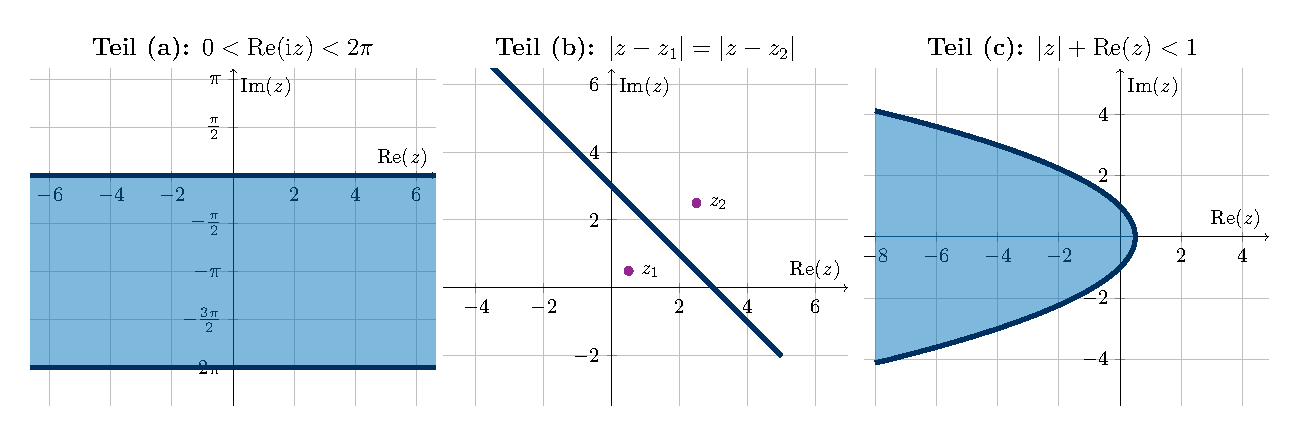
\includegraphics[width=\linewidth]{./fkt_uebungen-1-abb-abc.pdf}
	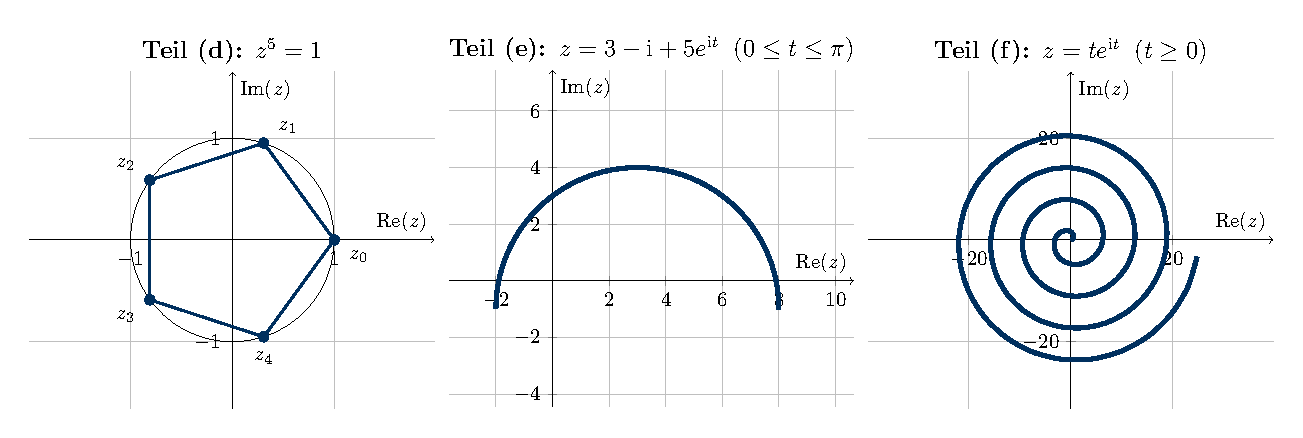
\includegraphics[width=\linewidth]{./fkt_uebungen-1-abb-def.pdf}
	\caption{Darstellungen zu \cref{task: 1.1}}
\end{figure}

\begin{task}
	Sei $\Omega \subseteq \CC$ offen, $z_0 \in \CC$, $\abb{f}{\Omega}{\CC}$.
	\begin{enumerate}[leftmargin=*, nolistsep, topsep=-\parskip]
		\item Zeigen Sie: $f$ ist genau dann in $z_0$ differenzierbar, wenn es $a \in \CC$ und $\abb{\phi}{\Omega}{\CC}$ mit $\lim_{z \to z_0} \phi(z) = 0$ gibt, sodass
		\begin{equation*}
			f(z) = f(z_0) + a (z-z_0) + \abs{z-z_0} \phi(z) \qquad (z \in \Omega)
		\end{equation*}
		gilt. Es ist dann $f'(z_0) = a$.
		\item Sei $\Omega' \subseteq \CC$ offen, $\abb{g}{\Omega'}{\CC}$, $f(\Omega) \subseteq \Omega'$ und seien $f$ in $z_0$ und $g$ in $f(z_0)$ differenzierbar. Zeigen Sie, dass $g \circ f$ in $z_0$ differenzierbar ist und dass
		\begin{equation*}
			(g \circ f)'(z_0) = g'(f(z_0)) * f'(z_0)
		\end{equation*}
		gilt (Kettenregel).
	\end{enumerate}
\end{task}

\pagebreak

\begin{enumerate}[leftmargin=*, label=(zu \alph*)]
	\item \begin{equivalence}
		\hinrichtung $f$ sei komplex differenzierbar in $z_0$, d.h. $f'(z_0)$ existiert. Definieren wir $a \defeq f'(z_0)$ und 
		\begin{equation*}
			\phi(z) \defeq \frac{z-z_0}{\abs{z-z_0}} * \schlange{\phi}(z) \quad \mit \quad  \schlange{\phi}(z) \defeq  \frac{f(z) - f(z_0)}{z-z_0} - f'(z_0)
		\end{equation*}
		Dann ist
		\begin{equation*}
			\begin{array}{rl}
			&f(z_0) + a(z-z_0) + \abs{z-z_0} \phi(z) \\
			=& 	f(z_0) + f'(z_0) * (z-z_0) + \abs{z-z_0} * \frac{z-z_0}{\abs{z-z_0}} * \brackets{\frac{f(z) - f(z_0)}{z-z_0}  - f'(z_0)}  \\
			=& f(z_0) + f'(z_0) * (z-z_0) + f(z) - f(z_0)  - f'(z_0) (z-z_0) \\
			=& f(z)
			\end{array}
		\end{equation*}
		Außerdem gilt aufgrund der Differenzierbarkeit von $f$ auch $\schlange{\phi}(z) \to 0$ für $z \to z_0$ sowie
		\begin{equation*}
			\abs{\frac{z-z_0}{\abs{z-z_0}}} = \frac{\abs{z-z_0}}{\abs{z-z_0}} = 1
		\end{equation*}
		und somit ist der Ausdruck $\frac{z-z_0}{\abs{z-z_0}}$ beschränkt. Schließlich dominiert somit $\schlange{\phi}$ die Konvergenz von $\phi$ und es gilt
		\begin{equation*}
			\lim_{z \to z_0} \phi(z) = 0
		\end{equation*}
		%
		\rueckrichtung Es existieren $a \in \CC$ und $\abb{\phi}{\CC}{\CC}$ mit $\phi(z) \to 0$ und $f(z) = f(z_0) + a * f'(z_0) (z-z_0) + \abs{z-z_0} * \phi(z)$. Daraus lässt sich umstellen
		\begin{align*}
				\frac{f(z) - f(z_0)}{z-z_0} 
				&= a + \phi(z) * \abs{z-z_0} * \frac{\quer{z-z_0}}{\quer{z-z_0}} \\
				&= a + \phi(z) * (z-z_0) * \frac{\quer{z-z_0}}{\abs{z-z_0}} \tag{$\frac{\abs{z}}{\quer{z}} = \frac{z}{\abs{z}}$}\\
				\follows \frac{f(z) - f(z_0)}{z-z_0} &= a + \phi(z) * \frac{\quer{z-z_0}}{\abs{z-z_0}}
		\end{align*}
		Somit ist 
		\begin{equation*}
			\lim_{z \to z_0} \frac{f(z) - f(z_0)}{z-z_0} = a + \lim_{z \to z_0} \underbrace{\phi(z) * \frac{\quer{z-z_0}}{\abs{z-z_0}}}_{\defqe \schlange{\phi}(z)}
		\end{equation*}
		Wie oben ist
		\begin{equation*}
			\abs{\frac{\quer{z-z_0}}{\abs{z-z_0}}} = \frac{\abs{z-z_0}}{\abs{z-z_0}} = 1
		\end{equation*}
		und somit dominiert $\phi$ den Ausdruck $\schlange{\phi}$ zu Null, d.h.
		\begin{equation*}
			\lim_{z \to z_0} \frac{f(z) - f(z_0)}{z-z_0} = a + \lim_{z \to z_0} \schlange{\phi}(z) = a \follows a = f'(z_0)
		\end{equation*}
	\end{equivalence}
	%
\pagebreak
	%
	\item Es seien $\abb{f}{\Omega}{\CC}$ in $z_0$ und $\abb{g}{\Omega'}{\CC}$ in $f(z_0)$ komplex differenzierbar.
	Dann gilt
	\begin{align*}
			\lim_{z \to z_0} \frac{(g \circ f) (z) - (g \circ f)(z_0)}{z - z_0}
			&= \lim_{z \to z_0} \frac{(g \circ f) (z) - (g \circ f)(z_0)}{f(z) - f(z_0)} * \frac{f(z) - f(z_0)}{z - z_0} \\
			&= \lim_{z \to z_0} \frac{(g \circ f) (z) - (g \circ f)(z_0)}{f(z) - f(z_0)} * \lim_{z \to z_0} \frac{f(z) - f(z_0)}{z - z_0} \\
			&= g'(f(z_0)) * \lim_{z \to z_0} \frac{f(z) - f(z_0)}{z - z_0} \tag{$g$ diffbar in $f(z_0)$} \\
			&= g'(f(z_0)) * f'(z_0) \tag{$f$ diffbar in $z_0$} 
	\end{align*}
	Insbesondere existieren die Grenzwerte $\lim_{z \to z_0} \frac{(g \circ f) (z) - (g \circ f)(z_0)}{f(z) - f(z_0)}$ und $\lim_{z \to z_0} \frac{f(z) - f(z_0)}{z - z_0}$ und somit auch der Grenzwert $\lim_{z \to z_0} \frac{(g \circ f) (z) - (g \circ f)(z_0)}{z - z_0}$, d.h. $g \circ f$ ist komplex differenzierbar in $z_0$.
\end{enumerate}

\begin{task}
	Seien $\abb{f,g,h}{\CC}{\CC}$ definiert durch
	\begin{equation*}
		\begin{aligned}
		f(z) &\defeq x^2 + y^2 \\
		g(z) &\defeq 2xy + y + \i (x^2 - y^2 - x) \\
		h(z) &\defeq \frac{x - \i y}{1 + x^2 + y^2}
		\end{aligned}
	\end{equation*}
	Bestimmten Sie die Punkte in $\CC$, in denen $f$, $g$ und $h$ komplex differenzierbar sind.
\end{task}

Wir zerlegen die Funktionen immer in Real- und Imaginärfunktion, d.h. $f(z) = f(x,y) = f_1(x,y) + \i * f_2(x,y)$. Damit ist $f_1(x,y) = x^2 + y^2$ und $f_2(x,y) = 0$. Für die partiellen Ableitungen gilt
\begin{align*}
	\partial_x f_1(x,y)  &= 2x 	&	\partial_y f_1(x,y) &= 2y \\
	\partial_x f_2(x,y)  &= 0 	&	\partial_y f_2(x,y) &= 0
\end{align*}
Alle partiellen Ableitungen sind stetig, somit ist $\abb{f}{\R^2}{\R^2}$ (reell) differenzierbar. Wir prüfen die Cauchy-Riemann-Differentialgleichungen:
\begin{equation*}
	\begin{array}{rcrcrcrcrcr}
	\partial_x f_1(x,y) &=& \partial_y f_2(x,y) &\equivalent& 2x &=& 0 &\equivalent& x &=& 0 \\
	\partial_y f_1(x,y) &=& - \partial_x f_2(x,y)  &\equivalent& 2y &=& 0 &\equivalent& y &=& 0 
	\end{array}
\end{equation*}
Damit sind die beiden Gleichungen nur für $z = 0$ erfüllt und $f$ ist nur in diesem Punkt komplex differenzierbar.

Es ist $g_1(x,y) = 2xy + y$ und $g_2(x,y) = x^2 - y^2 - x$. Für die partiellen Ableitungen gilt
\begin{align*}
	\partial_x g_1(x,y)  &= 2y 		&	\partial_y g_1(x,y) &= 2x+1 \\
	\partial_x g_2(x,y)  &= 2x-1	&	\partial_y g_2(x,y) &= -2y
\end{align*}
Alle partiellen Ableitungen sind stetig, somit ist $\abb{f}{\R^2}{\R^2}$ (reell) differenzierbar. Wir prüfen die Cauchy-Riemann-Differentialgleichungen:
\begin{equation*}
\begin{array}{rcrclclcrcr}
	\partial_x g_1(x,y) &=& \partial_y g_2(x,y) &\equivalent& 2y &=& -2y &\follows& y &=& 0 \\
	\partial_y g_1(x,y) &=& - \partial_x g_2(x,y)  &\equivalent& 2x+1 &=& -2x+1 &\follows& x &=& 0 
\end{array}
\end{equation*}
Damit sind die beiden Gleichungen nur für $z = 0$ erfüllt und $g$ ist nur in diesem Punkt komplex differenzierbar.

Es ist $h_1(x,y) = \frac{x}{1 + x^2 + y^2}$ und $h_2(x,y) = - \frac{y}{1 + x^2 + y^2}$. Für die partiellen Ableitungen gilt
\begin{align*}
	\partial_x h_1(x,y)  &= \frac{1-x^2+y^2}{(1 + x^2 + y^2)^2}	&	\partial_y h_1(x,y) &= \frac{-2xy}{(1 + x^2 + y^2)^2} \\
	\partial_x h_2(x,y)  &= \frac{-2xy}{(1 + x^2 + y^2)^2}		&	\partial_y h_2(x,y) &= -\frac{1+x^2-y^2}{(1 + x^2 + y^2)^2}
\end{align*}
Alle partiellen Ableitungen sind stetig für $x \neq \pm \sqrt{-y^2-1}$, somit ist $\abb{f}{\R^2}{\R^2}$ dort (reell) differenzierbar. Wir prüfen die Cauchy-Riemann-Differentialgleichungen:
\begin{equation*}
\begin{array}{rcrcccrcl}
	\partial_x h_1(x,y) &=& \partial_y h_2(x,y) &\equivalent& \frac{1-x^2+y^2}{(1 + x^2 + y^2)^2} = -\frac{1+x^2-y^2}{(1 + x^2 + y^2)^2} &\follows& 1 &=& -1 \\
	\partial_y h_1(x,y) &=& - \partial_x h_2(x,y)  &\equivalent& \frac{-2xy}{(1 + x^2 + y^2)^2} = \frac{2xy}{(1 + x^2 + y^2)^2} &\follows& -2xy &=& 2xy
\end{array}
\end{equation*}
Die erste Gleichung liefert aufgrund der falschen Aussage für alle $x,y \in \R$ die Unlösbarkeit des Gleichungssystems. Somit ist $h$ nirgends komplex differenzierbar.

\end{exercisePage}
\begin{exercisePage}
	
	\begin{task}
		Sei $\Omega \defeq B(0,1) \subseteq \CC$ (Einheitskreis), $\abb{f}{\Omega}{\CC}$, $f(\Omega) \subseteq \R$. Zeigen Sie: Ist $z_0 \in \Omega$, $f$ komplex differenzierbar in $z_0$, dann gilt $f'(z_0) = 0$. Ist $f$ (in $\Omega$) holomorph, so ist $f$ konstant.
	\end{task}
	
	Sei $f \simeq (u,v)$, $f = u + \i v$ und $z=x + \i y \simeq (x,y)$. Wegen $f(\Omega) \subseteq \R$ ist $v \equiv 0$. Da $f$ in $z_0 = x_0 + \i y_0 \simeq (x_0, y_0)$ komplex differenzierbar ist, ist $\abb{f}{\R^2}{\R}$ dort auch reell differenzierbar und es gelten die Cauchy-Riemann Differentialgleichungen $u_x(x_0,y_0) = v_y(x_0, y_0) = 0$ bzw. $u_y(x_0, y_0) = -v_x(x_0, y_0) = 0$. Somit ist auch $u'(z) = 0$ und somit $f'(x_0,y_0) \simeq f'(z_0) = 0$.
	
	Sei $f$ holomorph auf $\Omega$. Dann gilt $f'(z) = 0$ für alle $z \in \Omega$, insbesondere ist $u',v' \equiv 0$ und dann sind $u$ und $v$ als reelle Funktionen konstant, also auch $f  = u + \i  v$.
	
	
	\begin{task}
		\begin{enumerate}[label=(\alph*), nolistsep]
			\item Weisen Sie nach, dass die Funktion 
			\begin{equation*}
				\abb{u}{\R^2}{\R} \qquad u(x,y) \defeq e^{-x} (x * \cos(y) + y * \sin(y))
			\end{equation*}
			der Laplace-Differentialgleichung $\Delta u = u_{xx} + u_{yy}  = 0$ genügt.
			\item Bestimmen Sie eine Funktion $\abb{v}{\R^2}{\R}$ mit $v(0,0) = 0$ derart, dass $u$,$v$ die Cauchy-Riemann-Differentialgleichungen erfüllen.
			\item Schreiben Sie $f = u + \i v$ mithilfe der komplexen Exponentialfunktionen als Funktion von $z = x + \i y$.
		\end{enumerate}
	\end{task}

	\begin{enumerate}[label=(zu \alph*), leftmargin=*]
		\item Es ist
		\begin{align*}
			u_x(x,y) &= -e^{-x} \brackets{x * \cos(y) + y*\sin(y)} + e^{-x} * \cos(y) \\
			&= e^{-x} \brackets{(1-x) \cos(y) - y \sin(y)} \\
			u_{xx}(x,y) &= e^{-x} \brackets{x \cos(y) + y\sin(y) - 2\cos(y)} \\
			&= e^{-x} \brackets{(x-2) \cos(y) + y \sin(y)} \\
			u_y(x,y) &= e^{-x} \brackets{-x \sin(y) + \sin(y) + y \cos(y)} \\
			&= e^{-x} \brackets{(1-x) \sin(y) + y \cos(y)} \\
			u_{yy}(x,y) &= e^{-x} \brackets{-x \cos(y) + \cos(y) + \cos(y) - y\sin(y)} \\
			&= -e^{-x} \brackets{(x-2) \cos(y) + y \sin(y)}
		\end{align*}
		Damit gilt $u_{xx} + u_{yy} = 0$.
		\item Es gilt $u_x(x,y) = e^{-x} \brackets{(1-x) \cos(y) - y \sin(y)}$ und nach den Cauchy-Riemann Differentialgleichungen muss $u_x = v_y$ gelten. Löse diese Differentialgleichung für fixiertes $x$ durch Integration:
		\begin{equation*}
			\begin{aligned}
				v(x,y) &= \int u_x(x,y) \diffskip{y} = \int e^{-x} \brackets{(1-x) \cos(y) - y \sin(y)} \diffskip{y} \\
				&= e^{-x} \brackets{ (1-x) \int \cos(y) \diffskip{y} - \int y \sin(y) \diffskip{y}} \\
				&= e^{-x} \brackets{(1-x) \sin(y) - \sin(y) + y \cos(y) + C} \\
				&= e^{-x} \brackets{ -x \sin(y) + y \cos(y) + C} 
			\end{aligned}
		\end{equation*}
		Prüfen wir die zweite Cauchy-Riemann-Differentialgleichung und bestimmten $v_x$:
		\begin{equation*}
			\begin{aligned}
				v_x &= - e^{-x} \brackets{ -x \sin(y) + y \cos(y) + C} + e^{-x} (- \sin(y)) \\
				&= -e^{-x} \brackets{ (1-x) \sin(y) + y \cos(y) + C} \\
				\overset{!}&{=} u_y(x,y) \\
				&= -e^{-x} \brackets{(1-x) \sin(y) + y \cos(y)}
			\end{aligned}
		\end{equation*}
		Daraus erhalten wir die Konstante $C = 0$ und als Lösung $v(x,y) = e^{-x} \brackets{y\cos(y) - x\sin(y)}$. Auch der Anfangswert $v(0,0) = 1 * (0-0) = 0$ wird erfüllt.
		Die Probe ergibt
		\begin{equation*}
			\begin{aligned}
				v_x(x,y) 
				&= -e^{-x} \brackets{ -x \sin(y) + y \cos(y)} - e^{-x} \sin(y)\\
				&= -e^{-x} \brackets{(1-x) \sin(y) + y \cos(y)} = -u_y(x,y) \\
				v_y(x,y) &= e^{-x} \brackets{(-x \cos(y) + \cos(y) - y \sin(y))} \\
				&= e^{-x} \brackets{(1-x) \cos(y) - y \sin(y)} = u_x(x,y)
			\end{aligned}
		\end{equation*}
		also $u_x = v_y$ und $u_y = - v_x$.
		\item Sei $z = x + \i y$.
		\begin{equation*}
			\begin{aligned}
				f(x,y) &= u(x,y) + \i * v(x,y) \\
				&= e^{-x} \brackets{x * \cos(y) + y * \sin(y) - \i * x \sin(y) + \i * y \cos(y)} \\
				&= e^{-x} \brackets{(x + \i y) \cos(y) - \i * (x + \i y) \sin(y)} \\
				&= e^{-x} * z * \brackets{\cos(-y) + \i \sin(-y)} \\
				&= z * e^{-x} * e^{- \i y} \\
				&= z *e^{-z}
				= f(z)
			\end{aligned}
		\end{equation*}
	\end{enumerate}
	\begin{task}
		Sei $\Omega \subseteq \CC$ offen, $\abb{f}{\Omega}{\CC}$ holomorph, $f'$ stetig, $z_0 \in \Omega$, $f'(z_0) \neq 0$. Zeigen Sie: Es gibt offene Umgebungen $U \subseteq \Omega$ von $z_0$ und $V \subseteq \CC$ von $f(z_0)$, sodass $\abb{f}{U}{V}$ bijektiv und die daher existierende Abbildung $\abb{f^{-1}}{V}{U}$ ebenfalls holomorph ist. Es gilt $(f^{-1})'(w) = \frac{1}{f'(f^{-1}(w))}$ für alle $w \in V$. \\
		\textit{Hinweis:} Betrachten Sie $f = (f_1, f_2)$ als Abbildung von $\R^2$ nach $\R^2$. Deren Jabobi Determinante ist in $z_0 = (x_0, y_0)$ ungleich Null. Anwendung des Satzes über die lokale Invertierbarkeit.
	\end{task}

	Wir erinnern uns gemäß Hinweis an zwei Sätze aus der Analysis 2:
	
	\begin{lemma}[Satz über inverse Funktionen] \label{2lemma: invFkt}
		Sei $\abb{f}{U \subseteq \K^n}{\K^n}$ mit $\K \in \menge{\R, \CC}$ stetig differenzierbar ($U$ offen), $x_0 \in U$, $f'(x_0)$ regulär. Dann existiert eine offene Umgebung $U_0 \subseteq U$ von $x_0$, sodass mit $V_0 \defeq f(U_0)$ die eingeschränkte Abbildung $\abb{f}{U_0}{V_0}$ Diffeomorphismus\footnote{$f$, $f^{-1}$ stetig differenzierbar} ist (insbesondere ist $V_0$ offene Umgebung von $y_0 \defeq f(x_0)$).
	\end{lemma}
	\begin{lemma}[Ableitung der inversen Funktion] \label{2lemma: AbleitunginvFkt}
		Sei $\abb{f}{U \subseteq \K^n}{\K^n}$ injektiv und differenzierbar ($D$ offen, $\K \in \menge{\R, \CC}$), $f^{-1}$ differenzierbar in $y \in \inn(f(D))$. Dann ist
		\begin{equation*}
			(f^{-1})'(y) = f'(f^{-1}(y))^{-1}
		\end{equation*}
	\end{lemma}

	Sei $\abb{f = (f_1, f_2)}{\R^2}{\R^2}$ und $z = x + \i y \simeq (x,y)$ sowie $z_0 = x_0 + \i  y_0 \simeq (x_0,y_0)$. Da $f$ holomorph ist in allen $z_0 \in \Omega$, ist $f$ auch reell differenzierbar in $(x_0, y_0)$ mit 
	\begin{equation*}
		f'(x_0, y_0) = \begin{pmatrix}
			\partial_x f_1(x_0, y_0) & \partial_y f_1(x_0, y_0) \\
			\partial_x f_2(x_0, y_0) & \partial_y f_2(x_0, y_0)
		\end{pmatrix} 
		\defqe J
	\end{equation*}
	Außerdem gelten die Cauchy-Riemann-Differentialgleichungen $\partial_x f_1(x_0, y_0) = \partial_y f_2(x_0, y_0)$ und $\partial_y f_1(x_0, y_0) = - \partial_x f_2(x_0, y_0)$. Damit besitzt $J$ die Form $J = \left( \begin{smallmatrix} a & -b \\ b & a \end{smallmatrix} \right)$ mit Determinante
	\begin{equation*}
		\det(J) = \det\begin{pmatrix} a & -b \\ b & a \end{pmatrix} = a^2 + b^2
	\end{equation*}
	Angenommen es gilt $\det(J) = a^2 + b^2 = 0$. Dann ist $a=0$ und $b=0$, d.h. $f'(x_0, y_0) = 0$ im Widerspruch zur Voraussetzung. Somit ist also $f'(z_0) \simeq f'(x_0,y_0) \neq 0$ für alle $z_0 \simeq (x_0, y_0) \in \Omega$.
	
	Außerdem ist $f'$ stetig. Nach dem Satz über inverse Funktionen (\cref{2lemma: invFkt}) existiert dann eine offene Umgebung $U \subseteq \R^2$ von $(x_0, y_0)$, sodass mit $V = f(U)$ (und insbesondere $f(x_0,y_0) \in V$) $\abb{f}{U}{V}$ ein Diffeomorphismus ist. Nach dem Satz über die Ableitung der inversen Funktion (\cref{2lemma: AbleitunginvFkt}) gilt dann 
	\begin{equation*}
		\begin{aligned}
			(f^{-1})'(x,y) &= f'(f^{-1}(x,y))^{-1} \\
			&= 
			\begin{pmatrix}
				\partial_x f_1(f^{-1}(x,y)) & \partial_y f_1(f^{-1}(x,y)) \\
				\partial_x f_2(f^{-1}(x,y)) & \partial_y f_2(f^{-1}(x,y))
			\end{pmatrix}^{-1} \\
			&=
			\frac{1}{\det(J(f^{-1}(x,y)))}
				\begin{pmatrix}
				\partial_y f_2(f^{-1}(x,y)) & \partial_x f_2(f^{-1}(x,y)) \\
				\partial_y f_1(f^{-1}(x,y)) & \partial_x f_1(f^{-1}(x,y))
			\end{pmatrix}
			\qquad \forall (x,y) \in V
		\end{aligned}
	\end{equation*} 
	Aufgrund der Cauchy-Riemann-Differentialgleichungen für $f$ ist $\det(J(f^{-1}(x,y))) = \partial_x f_1(f^{-1}(x,y)) * \partial_y f_2(f^{-1}(x,y)) - \partial_x f_2(f^{-1}(x,y)) * \partial_y f_1(f^{-1}(x,y)) \neq 0$ und
	\begin{equation*}
		\begin{aligned}
			\partial_y f_2(f^{-1}(x,y)) &=  \partial_x f_1(f^{-1}(x,y)) \\
			\partial_y f_1(f^{-1}(x,y)) &= -\partial_x f_2(f^{-1}(x,y))
		\end{aligned}
	\end{equation*}
	auch die Cauchy-Riemann-Differentialgleichungen für $f^{-1}$. Damit ist $f^{-1}$ komplex differenzierbar auf dem entsprechenden $V \subseteq \CC$ mit der Ableitung
	\begin{equation*}
		\begin{aligned}
			(f^{-1})'(w) &= \lim_{z \to w} \frac{f^{-1}(z) - \lim_{z \to w} f^{-1}(w)}{z-w} = \frac{f^{-1}(z) - f^{-1}(w)}{f(f^{-1}(z)) - f(f^{-1}(w))} \\
			&= \brackets{\lim_{z \to w} \frac{f(f^{-1}(z)) - f(f^{-1}(w))}{f^{-1}(z) - f^{-1}(w)}}^{-1} \\
			&= \brackets{f'(f^{-1}(w))}^{-1} \qquad \forall w \in V
		\end{aligned}
	\end{equation*}
\end{exercisePage}
\begin{exercisePage}
	
	\begin{task}
		Das Doppelverhältnis $[z_1, z_2, z_3, z_4]$ von verschiedenen Punkten $z_1, z_2, z_3, z_4 \in \CC_\infty$ ist folgendermaßen erklärt:
		\begin{equation*}
			[z_1, z_2, z_3, z_4] = \frac{(z_1 - z_3) (z_2 - z_4)}{(z_1 - z_4) (z_2 - z_3)} \qquad z_1, z_2, z_3, z_4 \in \CC
		\end{equation*}
		Ist $z_j = \infty$, so definieren wir das Doppelverhältnis als Grenzwert, z.B.
		\begin{equation*}
			[\infty, z_2, z_3, z_4] \defeq \lim_{z \to \infty} [z, z_2, z_3, z_4] = \frac{z_2 - z_4}{z_2 - z_3}
		\end{equation*}
		\begin{enumerate}[nolistsep]
			\item Sei $\abb{f}{\CC_\infty}{\CC_\infty}$ eine Möbius-Transformation. Beweisen Sie: Sind $z_1, z_2, z_3, z_4 \in \CC_\infty$ und $z_j \neq z_k$ für $j \neq k$, so gilt
			\begin{equation*}
				[z_1, z_2, z_3, z_4] = [f(z_1), f(z_2), f(z_3), f(z_4)]
			\end{equation*}
			\item Benutzen Sie (a) um zu zeigen: Sind drei verschiedene Punkte $z_1, z_2, z_3 \in \CC_\infty$ und drei verschiedene Punkte $w_1, w_2, w_3 \in \CC_\infty$ gegeben, so existiert genau eine Möbius-Transformation $\abb{f}{\CC_\infty}{\CC_\infty}$ mit der Eigenschaft $f(z_j) = w_j$ für $j=1,2,3$. Für $z \notin \menge{z_1, z_2, z_3}$ ist $f(z)$ gegeben durch
			\begin{equation*}
				[w_1, w_2, w_3, f(z)] = [z_1, z_2, z_3, z]
			\end{equation*}
		\end{enumerate}
	\end{task}

	\begin{enumerate}[label=(zu \alph*), leftmargin=*]
		\item Sei $\abb{f}{\CC_\infty}{\CC_\infty}$ eine Möbius-Transformation, d.h. es existieren $a,b,c,d \in \CC$ mit $ad - bc \neq 0$, sodass $f(z) = \frac{az + b}{cz + d}$. Wir definieren abkürzend $\alpha(z) \defeq cz + d$ und $\delta \defeq ad - bc$.
		Außerdem gilt 
		\begin{equation}
			[z_1, z_2, z_3, z_4] = [z_2, z_1, z_4, z_3] = [z_3, z_4, z_1, z_2] 
			\tag{$\star$} \label{3eq: 1}
		\end{equation}
		\begin{enumerate}[label=(\roman*), leftmargin=*]
			\item Für $x,y \in \CC$ gilt
			\begin{equation*}
				\begin{aligned}
					f(x) - f(y) = \frac{ax + b}{cx + d} - \frac{ay + b}{cy + d} 
					&= \frac{(ax + b) (cy + d) - (ay + b (cx + d))}{(cx + d)(cy + d)} \\
					&= \frac{ac x y + ad x + bc y + bd - ac x y - ad y - bc x  - bd}{\alpha(x) \alpha(y)} \\
					&= \frac{(x-y) * \delta}{\alpha(x) * \alpha(y)}
				\end{aligned} 
			\end{equation*}
			Damit ist dann
			\begin{equation*}
				\begin{aligned}
					[f(z_1), f(z_2), f(z_3), f(z_4)] 
					&= \frac{\Big( f(z_1) - f(z_3) \Big) * \Big( f(z_2) - f(z_4) \Big)}{\Big( f(z_1) - f(z_4) \Big) * \Big( f(z_2) - f(z_3 \Big)} \\
					&= \frac{(z_1 - z_3) * \delta * (z_2 - z_4) * \delta}{\alpha(z_1) * \alpha(z_3) * \alpha(z_2) * \alpha(z_4)} * \frac{\alpha(z_1) * \alpha(z_4) * \alpha(z_2) * \alpha(z_3)}{(z_1 - z_4) * \delta * (z_2 + z_3) * \delta} \\
					&= \frac{(z_1 - z_3) (z_2 - z_4)}{(z_1 - z_4) (z_2 - z_3)} \\
					&= [z_1, z_2, z_3, z_4] 
				\end{aligned}
			\end{equation*}
			
			\item Genau ein $z_k = \infty$ und $c \neq 0$. Wegen \eqref{3eq: 1} können wir oBdA annehmen, dass $z_1 = \infty$. Dann ist $f(z_1) = \frac{a}{c}$ und es gilt
			\begin{equation*}
				f(z_1) - f(z) = \frac{a}{c} - \frac{a z + b}{c z + d} 
				= \frac{ac z + ad - acz - bc}{c (c z + d)}
				= \frac{\delta}{c * \alpha(z)} \qquad \forall z \in \CC
			\end{equation*}
			Somit ist
			\begin{equation*}
				\begin{aligned}
					[f(z_1), f(z_2), f(z_3), f(z_4)] 
					&= \frac{\delta (z_2 - z_4) * c * \alpha(z_4) * c * \alpha(z_2) * \alpha(z_3)}{c * \alpha(z_3) * \alpha(z_2) * \alpha(z_4) * \delta * (z_2 - z_3)} \\
					&= \frac{z_2 - z_4}{z_2 - z_3} \\
					&= [z_1, z_2, z_3, z_4]
				\end{aligned}
			\end{equation*}
			
			Für $c = 0$ ist $f(z_1) = \infty$ und somit $f(z_1) - f(z) = \infty$ für alle $z \in \CC$, sowie $\alpha \equiv d$. Es gilt
			\begin{equation*}
				\begin{aligned}
					[f(z_1), f(z_2), f(z_3), f(z_4)] 
					= \frac{f(z_2) - f(z_4)}{f(z_2) - f(z_3)} 
					= \frac{z_2 - z_4}{z_2 - z_3} * \frac{\delta * d^2}{\delta * d^2}
					= [z_1, z_2, z_3, z_4]
				\end{aligned}
			\end{equation*}
			
			\item Es seien $z_1 = z_2 = \infty$. Dann ist $f(z_1) = f(z_2) = \frac{a}{c}$ für $c \neq 0$. Somit vereinfacht sich Fall (ii) weiter zu
			\begin{equation*}
				\begin{aligned}
					[f(z_1), f(z_2), f(z_3), f(z_4)] 
					&= \frac{\delta*\delta}{c * \alpha(z_3) * c * \alpha(z_4)} * \frac{c * \alpha(z_4) * c * \alpha(z_3)}{\delta * \delta} \\
					&= 1 \\
					&= [z_1, z_2, z_3, z_4]
				\end{aligned}
			\end{equation*}
			Für $c = 0$ ist $f(z_1) = f(z_2) = \infty$ und somit $[f(z_1), f(z_2), f(z_3), f(z_4)] = 1 = [z_1, z_2, z_3, z_4]$.
			
			Sei $z_1 = z_3 = \infty$, dann folgt die Aussage in beiden Fällen mit ähnlicher Rechnung wie oben.
			
			\item Analog zu den bisher gezeigten Fällen, rechnet man auch alle weiteren Fälle nach. 
		\end{enumerate}
		Damit erhält man schließlich für alle $z_k \in \CC_\infty$ ($k=1,2,3,4$) die Aussage $[z_1, z_2, z_3, z_4] = [f(z_1), f(z_2), f(z_3), f(z_4)]$.
		
		\item Wir konstruieren eine Möbius-Transformation $f$ mit $f(z_j) = w_j$ ($j=1,2,3$). Dazu betrachten wir das Doppelverhältnis $[z_1, z_2, z_3, z_4]$ als Funktion $\tau$ in $z$, d.h.
		\begin{equation*}
			\tau(z) \defeq [z_1, z_2, z_3, z] = \frac{(z_1 - z_3)(z_2 - z)}{(z_1 - z) (z_2 - z_3)} = \frac{-(z_1 - z_3) * z + (z_1 - z_3) z_2}{-(z_2 - z_3) + (z_2 - z_3) z_1}
		\end{equation*}
		Mit der zugeordneten Matrix $T \defeq \left( \begin{smallmatrix}
		-(z_1 - z_3) & (z_1 - z_3) z_2 \\
		-(z_2 - z_3) & (z_2 - z_3) z_1
		\end{smallmatrix} \right)$ und $\det(T) = (z_1 - z_3) (z_2 - z_3) (z_2 - z_1) \neq 0$, da $z_1 \neq z_2$ vorausgesetzt war, ist $\tau$ wieder eine Möbius-Transformation.
		Dabei gilt $\tau(z_1) = \infty$, $\tau(z_2) = 0$ und $\tau(z_3) = 1$. 
		Sei $\sigma$ nun das Doppelverhältnis der $w_k$ und $z$ als Funktion in $z$ aufgefasst:
		\begin{equation*}
			\sigma(z) \defeq [w_1, w_2, w_3, z] = \frac{-(w_1 - w_3) * z + (w_1 - w_3) w_2}{-(w_2 - w_3) + (w_2 - w_3) w_1}
		\end{equation*}
		Mit der gleichen Überlegung wie für $\tau$ ist auch $\sigma$ wieder eine Möbius-Transformation mit der zugeordneten Matrix $S \defeq \left( \begin{smallmatrix}
		-(w_1 - w_3) & (w_1 - w_3) w_2 \\
		-(w_2 - w_3) & (w_2 - w_3) w_1
		\end{smallmatrix} \right)$.
		Mit 
		\begin{equation*}
			S^{-1} = \frac{1}{w_1 + w_2}
			\begin{pmatrix}
				\frac{1}{w_1 - w_3} & -\frac{w_2}{w_2 - w_3} \\
				\frac{1}{w_1 - w_3} & -\frac{1}{w_2 - w_3}
			\end{pmatrix}
		\end{equation*}
		ist $\sigma^{-1}$ wieder eine Möbius-Transformation und die Verkettung $\sigma^{-1} \circ \tau$ ist gegeben durch die Matrix
		\begin{equation*}
			S^{-1} * T = \frac{1}{w_1 + w_2}
			\begin{pmatrix}
				\frac{1}{w_1 - w_3} & -\frac{w_2}{w_2 - w_3} \\
				\frac{1}{w_1 - w_3} & -\frac{1}{w_2 - w_3}
			\end{pmatrix}
			*
			 \begin{pmatrix}
			-(z_1 - z_3) & (z_1 - z_3) z_2 \\
			-(z_2 - z_3) & (z_2 - z_3) z_1
			\end{pmatrix}
			= \dots
		\end{equation*}
		Die zugehörige Möbius-Transformation $f \defeq \sigma^{-1} \circ \tau$ erfüllt dann (wie man mit tausend mal mehr nachrechnen einsehen kann) gerade die Bedingungen $f(z_k) = w_k$ ($k=1,2,3$) und $[z_1, z_2, z_3, z] = [w_1, w_2, w_3, z]$. 
		
		\begin{lemma}
			Sei $f$ eine Möbius-Transformation gegeben durch $f(z) = \frac{az + b}{cz + d}$ ($a,b,c,d \in \CC_\infty$) mit $f \neq \id$. Dann hat $f$ höchstens zwei Fixpunkte.
		\end{lemma}
		\begin{proof}
			Die Fälle $c = 0$ und $a = 0$ sind klar.
			Betrachte die Fixpunktgleichung $z = f(z) = \frac{az + b}{cz + d}$. Umstellen ergibt die Polynomgleichung zweiten Grades
			\begin{equation*}
				z ( cz + c) = c z^2 + cz = a z + b \equivalent 0 = c * z^2 + (c - a) z - b
			\end{equation*}
			die nach dem Fundamentalsatz der Algebra höchstens zwei verschiedene Lösungen besitzt. Damit kann die Möbius-Transformation $f$ maximal zwei Fixpunkte besitzen.
		\end{proof}
	
		Sei nun $\schlange{f}$ eine weitere Möbius-Transformation, die die Interpolationsbedingungen erfüllt. Dann ist $f^{-1}(\schlange{f}(z_k)) = f^{-1}(w_k) = z_k$ für alle $k = 1,2,3$. Somit hat $f^{-1} \circ \schlange{f}$ also drei Fixpunkte. Jedoch kann eine Möbius-Transformation nur zwei Fixpunkte besitzen, wenn sie nicht die Identität ist. Somit muss $f^{-1} \circ \schlange{f} = \id$ gelten, was äquivalent zu $\schlange{f} = f$ ist. Somit ist das die Interpolationsbedingungen erfüllende $f$ eindeutig bestimmt.
	\end{enumerate} 




	\pagebreak
	
	
	
	
	\begin{task}
		Für $z \in \Omega \defeq \CC \setminus (-\infty, 0]$ sei der Hauptwert $\Arg(z)$ des Argumentes von $z$ festgelegt durch $- \pi < \Arg(z) < \pi$ (Das Argument $\phi$ von $z$ ist modulo $2\pi$ definiert durch $z = \abs{z} + e^{i\phi}$). Wir definieren $\abb{\Ln}{\Omega}{\CC}$ durch
		\begin{equation}
			\Ln(z) \defeq \ln\abs{z} + \i * \Arg(z) \tag{Hauptzweig des Logarithmus}
		\end{equation}
		Beweisen Sie:
		\begin{enumerate}
			\item $\Ln$ ist die Umkehrfunktion von $\abb{\exp}{\menge{z \in \CC : - \pi < \Im(z) < \pi}}{\Omega}$.
			\item $\Ln$ ist holomorph. (Hinweis: Aufgabe 2.3)
		\end{enumerate}
	\end{task}

	\begin{enumerate}[label=(zu \alph*), leftmargin=*]
		\item Sei $z \in \Omega$. Dann existiert $\phi \in (-\pi,\pi)$, sodass $z = \abs{z} * e^{i\phi}$, d.h. $\phi = \Arg(z)$. Es ist $\Im(\Ln(z)) = \Arg(z) = \phi \in (-\pi, \pi)$. Somit können wir $\exp$ anwenden und erhalten
		\begin{equation*}
			\exp(\Ln(z)) = \exp(\ln \abs{z}) * \exp(\i * \phi) = \abs{z} * e^{i \phi} = z
		\end{equation*} 
		Umgekehrt sei $z \in \menge{z \in \CC : -\pi < \Im(z) < \pi}$. Dann gilt mit $z = a + b \i$ und $b \in (-\pi, \pi)$ auch $\exp(a + b \i) = \exp(a) * \exp(b \i) \in \Omega$. Somit gilt
		\begin{equation*}
			\begin{aligned}
				\Arg(\exp(a + b \i)) &= \Arg( \exp(a) * \exp(b \i) ) = b \\
				\ln \abs{\exp(a + b \i)} &= \ln(\exp(a)) * \ln \abs{\exp(b \i)} = a
			\end{aligned}
		\end{equation*}
		und schließlich
		\begin{equation*}
			\Ln(\exp(z)) = \ln \abs{\exp(a + b \i)} + \i * \Arg(\exp(a + b \i)) = a + b \i = z
		\end{equation*}
		Somit ist $\exp \circ \Ln = \id = \Ln \circ \exp$ und $\Ln$ die Umkehrung von $\exp$ als Abbildungen zwischen $\Omega$ und $\menge{z \in \CC : - \pi < \Im(z) < \pi}$.
		
		\item Wir wissen, dass $\exp$ auf $\CC$ stetig und holomorph ist mit $\exp'(z_0) = \exp(z_0) \neq 0$ für alle $z_0 \in \CC$. Nach Aufgabe 2.3 existieren dann offene Umgebungen $U$ von $z_0$ und $V$ von $\exp(z_0)$, sodass $\abb{\exp}{U}{V}$ ein Diffeomorphismus ist. 
		Wir wissen außerdem, dass $\exp$ auf $\Omega' \defeq \menge{z \in \CC : - \pi < \Im(z) < \pi}$ injektiv ist, d.h. wir können jede beliebige offene Umgebung $U \subseteq \Omega'$ mit $z_0 \in U$ wählen und erhalten mit $V = \exp(U) \subseteq \Omega$ eine offene Umgebung von $\exp(z_0)$. Somit ist die Umkehrabbildung $\abb{\Ln}{V}{U}$ auf allen offenen $V \subseteq \Omega$ holomorph, d.h. auch auf $\Omega$ selbst.
	\end{enumerate}



	\pagebreak
	
	

	\begin{task}
		\begin{enumerate}
			\item Finden Sie $z_1, z_2 \in \CC \setminus (-\infty, 0]$, sodass $\Ln(z_1 * z_2) \neq \Ln(z_1) + \Ln(z_2)$.
			\item Sei $z_1 \in \CC \setminus (-\infty, 0]$ mit $\Re(z_1) = 0$ und $\Im(z_1) > 0$. Finden Sie alle $z_2 \in \CC \setminus (-\infty, 0]$, für die $\Ln(z_1 * z_2) = \Ln(z_1) + \Ln(z_2)$ gilt.
		\end{enumerate}
	\end{task}

	\begin{enumerate}[label=(zu \alph*), leftmargin=*]
		\item Sei $z_1 = \i$ und $z_2 = \i - 1$. Dann sind offensichtlich $z_1, z_2 \in \CC \setminus (-\infty, 0]$. Es gilt
		\begin{align*}
				\Ln(\i) &= \ln\abs{\i} + \i * \Arg(\i) = 0 + \i * \frac{\pi}{2} \\
				\Ln(\i - 1) &= \ln\abs{\i - 1} + \i * \Arg(\i - 1) = \ln(\sqrt{2}) + \i * \frac{3}{4} \pi \\
			\intertext{Aber}
				\Ln(\i * (\i - 1)) &= \Ln(-\i  - 1) = \ln \abs{i + 1} + \i * \Arg(-\i - 1) = \ln(\sqrt{2}) - \i * \frac{3}{4} \pi \\
				\Ln(i) + \Ln(i-1) &= \ln(\sqrt{2}) + \i * \frac{3}{4} \pi + \i * \frac{\pi}{2} = \ln(\sqrt{2}) + \i * \frac{5}{4} \pi
		\end{align*}
		Wegen $\Ln(\i) + \Ln(\i-1) - \Ln(\i * (\i - 1)) = \i * \frac{1}{2} \pi \neq 0$ ist $\Ln(z_1 * z_2) \neq \Ln(z_1) + \Ln(z_2)$.
		
		\item Sei $z_k = r_k * e^{\i \phi_k}$ für $k = 1,2$ und wegen $\Re(z_1) = 0$ sowie $\Im(z_1) > 0$ gilt $r_1 > 0$ und $\phi_1 = \frac{\pi}{2}$. Notiere daher im Folgenden $\phi \defeq \phi_2$. Es gilt
		\begin{equation*}
			\Ln(z_1 z_2) = \ln{\abs{r_1 r_2 * e^{\i (\phi + \frac{\pi}{2})}}} + \i * \Arg\brackets{r_1 r_2 * e^{\i (\phi + \frac{\pi}{2})}} = \ln \abs{r_1 r_2} + \i * \brackets{\phi + \frac{\pi}{2} \mod 2\pi}
		\end{equation*}
		und 
		\begin{equation*}
		\begin{aligned}
				\Ln(z_1) + \Ln(z_2) &= \ln\abs{r_1 e^{i \frac{\pi}{2}}} + \i * \Arg\brackets{r_1 e^{i \frac{\pi}{2}}} + \ln\abs{r_2 e^{i \phi}} + \i * \Arg\brackets{r_2 e^{i \phi}} \\
				&= \ln\abs{r_1 r_2} + \i * \brackets{\frac{\pi}{2} + \phi}
		\end{aligned}
		\end{equation*}
		Setzen wir nun beide Ausdrücke gleich, so erhalten wir
		\begin{equation*}
			\begin{aligned}
			\ln \abs{r_1 r_2} + \i * \brackets{\phi + \frac{\pi}{2} \mod 2\pi} &= \ln\abs{r_1 r_2} + \i * \brackets{\frac{\pi}{2} + \phi} \\
			\equivalent \qquad \phi + \frac{\pi}{2} \mod 2\pi &= \frac{\pi}{2} + \phi
			\end{aligned}
		\end{equation*}
		Diese Gleichung wird für alle $\phi + \frac{\pi}{2} \in (-\pi, \pi)$ erfüllt. Da aber auch $\phi \in (-\pi, \pi)$ als Hauptwert gilt, schränkt sich diese beiden Bedingungen gegenseitig ein zu $\phi \in \brackets{-\pi, \frac{\pi}{2}}$. Somit gilt die Gleichheit der zu zeigenden Aussage für alle $z_2 = \abs{z_2} * e^{\i \phi}$ mit $\phi \in \brackets{-\pi, \frac{\pi}{2}}$
	\end{enumerate}
\end{exercisePage}
\begin{exercisePage}
	
	\begin{task}
		Berechnen Sie das Integral $\int_\gamma \abs{z} * \quer{z} \diff{z}$ folgende Wege $\gamma$ mit Anfangspunkt $-1$ und Endpunkt $+1$.
		\begin{enumerate}[nolistsep]
			\item geradlinige Verbindung
			\item obere Halbkreislinie
			\item untere Halbkreislinie
		\end{enumerate}
	\end{task}

	\begin{enumerate}[label=(zu \alph*), leftmargin=*]
		\item Sei $f(z) \defeq \abs{z} * \quer{z}$. Parametrisiere die geradlinige Verbindungsstrecke durch den Weg $\abb{\gamma}{[-1,1]}{\CC}$ mit $\gamma(t) = t$ für alle $t \in [-1,1]$. Dann ist $\gamma'(t) = 1$ für $t \in [-1,1]$ und $f(\gamma(t))  = \abs{t} * \quer{t} = \sgn(t) * t^2$, da $t \in [-1,1] \subset \R$. Somit gilt also
		\begin{equation*}
			\int_\gamma \abs{z} \quer{z} \dz 
			= \int_{-1}^1 \sgn(t) * t^2 \dt 
			= \int_{-1}^0 -t^2 \dt + \int_0^1 t^2 \dt 
			= \sqbrackets{-\frac{1}{3}t^3}_{-1}^0 + \sqbrackets{\frac{1}{3}t^2}_0^1 
			= - \frac{1}{3} + \frac{1}{3} = 0
		\end{equation*}
		
		\item Parametrisiere den Weg durch $\abb{\gamma}{[0, \pi]}{\CC}$ mit $\gamma(t) = -e^{-\i t}$. Dann ist $\gamma'(t) = \i e^{-\i t}$ und $f(\gamma(t)) = \abs{\gamma(t)} * \quer{\gamma(t)} = \abs{- e^{- \i t}} * \brackets{-e ^{\i t}} = - e^{\i t}$. Somit gilt
		\begin{equation*}
			\int_\gamma \abs{z} \quer{z} \dz 
			= \int_0^\pi  - e^{\i t} * \i e^{-\i t} \dt 
			= -\i * \int_0^\pi 1 \dt
			= - \pi \i
		\end{equation*}
		
		\item Parametrisiere den Weg durch $\abb{\gamma}{[0, \pi]}{\CC}$ mit $\gamma(t) = -e^{\i t}$. Dann ist $\gamma'(t) = -\i e^{\i t}$ und $f(\gamma(t)) = \abs{\gamma(t)} * \quer{\gamma(t)} = \abs{- e^{\i t}} * \brackets{-e ^{-\i t}} = - e^{-\i t}$. Somit gilt
		\begin{equation*}
			\int_\gamma \abs{z} \quer{z} \dz 
			= \int_0^\pi   - e^{-\i t} * \brackets{-\i e^{\i t}} \dt 
			= \i * \int_0^\pi 1 \dt
			= \pi \i
		\end{equation*}
	\end{enumerate}

	\begin{task}
		Sei $\Omega \subseteq \CC$ offen, $\abb{f}{\Omega}{\CC}$ holomorph, $f'$ stetig und $\gamma$ ein stückweise stetig differenzierbarer Weg in $\Omega$. Zeigen Sie: $f \circ \gamma$ ist ein stückweise stetig differenzierbarer Weg in $\CC$ und für $\abb{g}{\Image (f \circ \gamma)}{\CC}$ stetig gilt
		\begin{equation*}
			\int_{f \circ \gamma} g(w) \diffskip{w} = \int_\gamma g(f(z)) * f'(z) \dz
		\end{equation*}
	\end{task}
	Sei $\gamma$ ein stückweise stetig differenzierbarer Weg auf dem Intervall $[a,b]$, d.h. es existiert eine Unterteilung $a = t_0 < t_1 < \dots < t_n = b$, sodass $\gamma|_{[t_i, t_{i+1}]}$ für alle $i \in \menge{1, \dots, n-1}$ stetig differenzierbar ist. Da $f$ als holomorphe Funktion stetig ist und $\gamma$ ein Weg, ist insbesondere auch $f \circ \gamma$ stetig, also ein Weg. Wir betrachten ein fixiertes Intervall $[t_i, t_{i+1}]$. Dort ist $f \circ \gamma$ nach Kettenregel differenzierbar mit $(f \circ \gamma)'(t) = f'(\gamma(t)) * \gamma'(t)$. Aufgrund der Stetigkeit von $f'$ und $\gamma'$ auf dem oben gewählten Intervall, ist auch $(f \circ \gamma)'$ stetig. Diese Betrachtung kann für jedes $i \in \menge{1, \dots, n-1}$ ausgeführt werden mit dem Ergebnis, dass $f \circ \gamma$ ein stückweise stetig differenzierbarer Weg ist. 
	Mit der oben ausgeführten Kettenregel und der Definition für Integrale über stückweise stetig differenzierbare Wege aus der Vorlesung gilt
	\begin{align*}
		\int_{f \circ \gamma} g(w) \diffskip{w} 
		&= \int_a^b g(f(\gamma(t))) * (f \circ \gamma)'(t) \dt \\
		&= \int_a^b (g \circ (f \circ \gamma))(t) * \brackets{f'(\gamma(t)) * \gamma'(t)} \dt \\
		&= \int_a^b \bigg( ((g \circ f)\circ \gamma)(t) * f'(\gamma(t)) \bigg) * \gamma'(t) \dt \\
		&= \int_\gamma (g \circ f)(z) * f'(z) \dz
	\end{align*}
	
	\begin{task}
		Für $\sigma \in \CC$ sei $\abb{f_\sigma}{\CC \setminus (- \infty, 0]}{\CC}$ definiert durch
		\begin{equation*}
			f_\sigma(z) \defeq \exp(\sigma \ \Ln(z))
		\end{equation*}
		mit dem Hauptzweig $\Ln$ des Logarithmus (siehe Aufgabe 3.2). Zeigen Sie:
		\begin{enumerate}
			\item Für $n \in \Z$ gilt $f_n(z) = z^n$ ($z \in \CC \setminus (-\infty, 0]$)
			\item Für alle $\sigma, \tau \in \CC$ gilt $f_\sigma * f_\tau = f_{\sigma + \tau}$.
			\item Für $\sigma \in [-1,1]$ und $\tau \in \CC$ gilt $f_\tau \circ f_\sigma = f_{\tau \sigma}$. Gilt dies auch für beliebige $\sigma \in \CC$.
			\item Für $\sigma \in \CC \setminus \N_0$ hat die binomische Reihe $b_\sigma(z) = \sum_{k=0}^{\infty} \binom{\sigma}{k} z^k$ den Konvergenzradius $1$.
			\item Für $\abs{z} < 1$ gilt $f_\sigma(1+z) = b_\sigma(z)$.			
		\end{enumerate}
		Hinweis: Taylor-Entwicklung von $z \mapsto f_\sigma(1+z)$ um $z=0$.
	\end{task}

	\begin{enumerate}[label=(zu \alph*), leftmargin=*]
		\item Sei $\phi = \Arg(z) \in (-\pi, \pi)$. Dann gilt $z = \abs{z} * e^{\i \phi}$. 
		\begin{equation*}
			f_n(z) = e^{n * (\ln\abs{z} + \i \Arg(z))} = \brackets{e^{\ln\abs{z}}}^n * \brackets{e^{\i \phi}}^n = \brackets{\abs{z} * e^{\i \phi}}^n = z^n
		\end{equation*}
		\item $(f_\sigma * f_\tau)(z) = \exp(\sigma \Ln(z)) * \exp(\tau \Ln(z)) = \exp((\sigma + \tau) \Ln(z)) = f_{\sigma + \tau}(z)$
		\item Sei $\sigma \in [-1,1]$ und $\tau \in \CC$. Dann gilt
		\begin{align*}
			(f_\tau \circ f_\sigma)(z) = e^{\tau \Ln\brackets{e^{\sigma \Ln(z)}}} 
			&= e^{\tau \Ln\brackets{e^{\sigma \ln\abs{z} + \sigma \i \Arg(z)}}} \\
			&= e^{\tau \ln\abs{e^{\sigma \ln\abs{z} + \sigma \i \Arg(z)}} + \tau \i \Arg\brackets{e^{\sigma \ln\abs{z} + \sigma \i \Arg(z)}}} \\
			&= e^{\tau \ln\abs{e^{\sigma \ln\abs{z}}} + \tau \i \Arg\brackets{e^{\sigma \i \Arg(z)}}} \tag{$\Im(\sigma) = 0$}\\
			&= e^{\sigma \tau \ln\abs{z} + \sigma \tau \i \Arg(z)} \tag{$\Re(\sigma) \le 1$}\\
			&= e^{\sigma \tau \brackets{\ln\abs{z} + \i \Arg(z)}} \\
			&= e^{\sigma \tau \Ln(z)} 
			= f_{\sigma \tau}(z)
		\end{align*}
		Da wir sowohl $\Im(\sigma) = 0$ als auch $\Re(\sigma) \le 1$ ausgenutzt haben, funktioniert der Beweis nicht für alle $\sigma \in \CC$.
		\item Sei $a_n \defeq \binom{\sigma}{n} = \prod_{j=1}^{n} \frac{\sigma - j + 1}{j}$. Dann gilt nach Quotientenkriterium für den Konvergenzradius $R$ von $b_\sigma(z)$
		\begin{equation*}
			R = \lim_{n \to \infty} \abs{\frac{a_n}{a_{n+1}}} = \lim_{n \to \infty} \abs{\frac{\prod_{j=1}^{n} \frac{\sigma - j + 1}{j}}{\prod_{j=1}^{n+1} \frac{\sigma - j + 1}{j}}} 
			= \lim_{n \to \infty} \abs{\frac{1}{\frac{\sigma -(n + 1) + 1}{n+1}}}
			= \lim_{n \to \infty} \abs{\frac{n+1}{\sigma - n}} = 1
		\end{equation*}
		\item Wir betrachten die Taylor-Entwicklung von $f_\sigma(1+z)$ um $z=0$. Es gilt für die Ableitungen
		\begin{equation*}
			f_\sigma^{(n)}(z) = \exp(\sigma \Ln(z)) * \brackets{\frac{1}{z^{n}} \prod_{j=1}^n (\sigma - j + 1)}
		\end{equation*} 
		Vollständige Induktion nach $n \in \N_0$:
		\begin{induction}
			\ianfang[$n=0$] Es ist $\exp(\sigma \Ln(z)) * \brackets{\frac{1}{z^0} \prod_{j=1}^0 (\sigma - j + 1)} = \exp(\sigma \Ln(z)) = f_\sigma^{(0)}(z)$.
			\ischritt Definiere $\phi_\sigma(n) \defeq \prod_{j=1}^n (\sigma - j + 1)$.
			\begin{align*}
				f_\sigma^{(n+1)}(z) 
				&= \ableitung{z} \brackets{\exp(\sigma \Ln(z)) * \brackets{\frac{1}{z^{n}} \phi_\sigma(n)}} \\
				&= \exp(\sigma \Ln(z)) * \frac{\sigma}{z} \brackets{\frac{1}{z^{n}} \phi_\sigma(n)} - \exp(\sigma \Ln(z)) \brackets{\frac{n}{z^{n+1}} \phi_\sigma(n)} \\
				&= \exp(\sigma \Ln(z)) \brackets{\frac{\sigma}{z^{n+1}} \phi_\sigma(n)} - \exp(\sigma \Ln(z)) \brackets{\frac{n}{z^{n+1}} \phi_\sigma(n)} \\
				&= \exp(\sigma \Ln(z)) \brackets{\frac{\sigma-n}{z^{n+1}} \phi_\sigma(n)} \\
				&= \exp(\sigma \Ln(z)) \brackets{\frac{1}{z^{n+1}} \phi_\sigma(n+1)} \\
				&= \exp(\sigma \Ln(z)) \brackets{\frac{1}{z^{n+1}} \prod_{j=1}^{n+1} (\sigma - j + 1)}
			\end{align*}
		\end{induction}
		Somit ist $f_\sigma^{(n)}(1) = \phi_\sigma(n) = \prod_{j=1}^n (\sigma - j + 1)$.
		Setzen wir dies in die Taylorreihe ein, so erhalten wir
		\begin{equation*}
			f_\sigma(1+z) = \sum_{n=0}^{\infty} \frac{f_\sigma^{(n)}(1)}{n!} z^n = \sum_{n=0}^{\infty} \prod_{j=1}^n \frac{\sigma - j + 1}{j} z^n 
			= \sum_{n=0}^{\infty} \binom{\sigma}{n} z^n 
			= b_\sigma(z)
		\end{equation*}
		für alle $\abs{z} < 1$.
	\end{enumerate}
\end{exercisePage}

\begin{exercisePage}[Kompakte Konvergenz, Integralberechnung, Nullhomologie \& --homotopie]
	
	\begin{task}
		Sei $\Omega \subseteq \Rn$ offen, $(f_n)$ eine Folge von stetigen Funktionen $\abb{f_n}{\Omega}{\CC}$ und $\abb{f}{\Omega}{\CC}$. Zeigen Sie die Äquivalenz folgender Aussagen:
		\begin{enumerate}[label=(\roman*), leftmargin=*, nolistsep]
			\item $(f_n)$ ist kompakt konvergent gegen $f$, d.h. gleichmäßig konvergent auf kompakten Teilmengen von $\Omega$: Für alle $K \subseteq \Omega$ kompakt mit $K \neq \emptyset$ gilt
			\begin{equation*}
				\sup\menge{\abs{f(\zeta) - f_n(\zeta)} : \zeta \in K} \to 0 \qquad (n \to \infty)
			\end{equation*}
			\item $(f_n)$ ist lokal gleichmäßig konvergent gegen $f$, d.h. für alle $z \in \Omega$ gibt es eine Umgebung $U \subseteq \Omega$ von $z$, sodass
			\begin{equation*}
				\sup\menge{\abs{f(\zeta) - f_n(\zeta)} : \zeta \in U} \to 0 \qquad (n \to \infty)
			\end{equation*}
		\end{enumerate}
	\end{task}
	
	\begin{equivalence}
		\hinrichtung Sei $f_n \to f$ kompakt und $z \in \Omega$. Da $\Omega$ offen ist, existiert eine Umgebung $B_\epsilon(z) \subseteq \Omega$ mit $\quer{B_\epsilon(z)} \subseteq \Omega$. Da $\quer{B_\epsilon(z)}$ beschränkt und abgeschlossen ist, ist $\quer{B_\epsilon(z)}$ kompakt. Nach Voraussetzung konvergiert also $f_n \to f$ gleichmäßig auf $\quer{B_\epsilon(z)}$, d.h. $\sup\menge{\abs{f(\zeta) - f_n(\zeta)} : \zeta \in \quer{B_\epsilon(z)}} \to 0$. Somit ist auch $\sup\menge{\abs{f(\zeta) - f_n(\zeta)} : \zeta \in B_\epsilon(z)} \to 0$ für alle $z \in \Omega$ und daher $f_n \to f$ lokal gleichmäßig.
		\rueckrichtung Sei $f_n \to f$ lokal gleichmäßig, d.h. für jedes $z \in \Omega$ existiert ein $\epsilon > 0$, sodass $B_\epsilon(z) \subseteq \Omega$ und $\sup\menge{\abs{f(\zeta) - f_n(\zeta)} : \zeta \in B_\epsilon(z)} \to 0$. Sei nun $K \subseteq \Omega$ eine beliebige kompakte Menge und $\folge{B_\epsilon(z)}{z \in K}$ eine offene Überdeckung von $K$ mit $f_n \to f$ gleichmäßig auf jeder Umgebung $B_\epsilon(z)$ ($z \in K$). Aufgrund der Kompaktheit von $K$ existiert eine endliche Teilüberdeckung $\menge{B_{\epsilon_i}(z_i)}_{i=1}^n$. Sei $\epsilon > 0$. Aufgrund der gleichmäßigen Konvergenz existiert dann für $1 \le i \le n$ ein $N_i$, sodass $\sup\menge{\abs{f(\zeta) - f_n(\zeta)} : \zeta \in B_\epsilon(z)} < \epsilon$ für alle $n > N_i$. Setze nun $N \defeq \max\menge{N_i : 1 \le i \le n}$ und $B \defeq \bigcup_{i=1}^n B_{\epsilon_i}(z_i)$. Dann ist $\sup\menge{\abs{f(\zeta) - f_n(\zeta)} : \zeta \in B} < \epsilon$ für alle $n > N$, d.h. $\sup\menge{\abs{f(\zeta) - f_n(\zeta)} : \zeta \in B} \to 0$ für $n \to \infty$. Somit konvergiert $f_n \to f$ gleichmäßig auf $B$, also auch auf dem beliebigen Kompaktum $K$ und daher ist $f_n$ kompakt konvergent gegen $f$.
	\end{equivalence}

	
	\begin{task}
		Sei $\abb{f}{\CC}{\CC}$ stetig und die Einschränkung von $f$ auf $\menge{z \in \CC : \Re(z) \neq 0}$ sei holomorph. Zeigen Sie, dass
		\begin{equation*}
			\int_{\triangle(a,b,c)} f(z) \dz = 0
		\end{equation*} 
		für alle $a,b,c \in \CC$. Mit dem Satz von Morera ist dann $f$ holomorph. 
		
		Hinweis: Zeigen Sie zuerst, dass $\int_\gamma f(z) \dz = 0$ für jeden geschlossenen Weg $\abb{\gamma}{[a,b]}{\menge{z \in \CC : \Re(z) \ge 0}}$.
	\end{task}

	\pagebreak

	Sei $\CC^+ \defeq \menge{z \in \CC : \Re(z) > 0}$ und $\quer{\CC^+} \defeq \menge{z \in \CC : \Re(z) \ge 0}$. Wir wollen zeigen, dass $\CC^+$ sternförmig ist, d.h. es existiert ein $z_0 \in \CC^+$, sodass $\im(\sigma_{z_0,z}) \subseteq \CC^+$ für alle $z \in \CC^+$. Wähle $z_0 = 1$. Dann ist für jeden Punkt $z$ der rechten Halbebene auch die Verbindungsstrecke $\im(\sigma_{z_0, z})$ in der rechter Halbebene. Für einen stückweise stetig differenzierbaren und geschlossenen Weg $\abb{\gamma}{[a,b]}{\quer{\CC^+}}$ betrachten wir den Weg $\gamma + \epsilon$ für ein $\epsilon > 0$. Dieser liegt dann vollständig in $\CC^+$. Dort ist $f$ holomorph und nach dem Cauchyschen Integralsatz gilt dann $\int_{\gamma + \epsilon} f(z) \dz = 0$. 
	
	Sei nun $\epsilon_n \to 0$. Definiere $f_n(\gamma(t)) \defeq f(\gamma(t) + \epsilon_n)$. Dann gilt wegen der Stetigkeit von $f$, dass $f_n(\gamma(t)) \to f(\gamma(t))$ für $n \to \infty$, d.h. $f(\gamma(t) + \epsilon) \to f(\gamma(t))$ für $\epsilon \to 0$.
	$\gamma$ ist stückweise stetig differenzierbar, d.h. wir betrachten eine Unterteilung $a = t_0 < t_1 < \dots < t_n = b$ und notieren $\mathcal{I}_i \defeq [t_i, t_{i+1}]$ für alle $i \in \menge{0, \dots, n-1}$. Aufgrund der Stetigkeit von $f$ und der Stetigkeit von $\gamma$ auf $\mathcal{I}_i$ ist $f \circ \gamma$ stetig auf kompaktem $\mathcal{I}_i$ für alle $i \in \menge{0, \dots, n-1}$. Somit existiert für alle $i \in \menge{0, \dots, n-1}$ eine integrierbare Konstante $c_i < \infty$, sodass $f_n(\gamma(t)) \le c_i$ für alle $t \in \mathcal{I}_i$. Definiere nun $c \equiv \max\menge{c_i : 0 \le i \le n-1}$. Damit ist $f_n(\gamma(t)) \le c$ für alle $t \in [a,b]$. Mit majorisierter Konvergenz erhalten wir also
	\begin{align*}
		\lim_{\epsilon \to 0} \int_a^b f(\gamma(t) + \epsilon) \dt
		&= \lim_{n \to \infty} \int_a^b f_n(\gamma(t)) \dt \tag{Grenzwert von Funktionen} \\
		&= \int_a^b \lim_{n \to \infty} f_n(\gamma(t)) \dt \tag{majorisierte Konvergenz}\\
		&= \int_a^b f(\gamma(t)) \dt \tag{Stetigkeit von $f$}
	\end{align*}
	
	Es ist damit
	\begin{align*}
			0 = \lim_{\epsilon \to 0} \int_{\gamma + \epsilon} f(z) \dz 
			= \lim_{\epsilon \to 0} \int_a^b f(\gamma(t) + \epsilon) * \gamma'(t) \dt 
			= \int_a^b f(\gamma(t)) * \gamma'(t) \dt 
			= \int_\gamma f(z) \dz
	\end{align*}
	Analog gilt dieses Resultat auch für alle Wege $\abb{\gamma}{[a,b]}{\quer{\CC^-}}$.
	
	Liegen nun $a$, $b$ und $c$ in der gleichen Halbebene $\quer{\CC^+}$ oder $\quer{\CC^-}$, dann lässt sich das Dreieck $\triangle(a,b,c)$ darstellen als geschlossener Weg in dieser Halbebene. Ohne Einschränkung seien $a,b,c \in \quer{\CC^+}$. Dann ist $\triangle(a,b,c) = \sigma_{a,b} \dot{+} \sigma_{b,c} \dot{+} \sigma_{c,a}$ in $\quer{\CC^+}$. Mithilfe des oben gezeigten Hinweises ist dann 
	\begin{equation*}
		\int_{\triangle(a,b,c} f(z) \dz = \int_{\sigma_{a,b} \dot{+} \sigma_{b,c} \dot{+} \sigma_{c,a}} f(z) \dz = 0
	\end{equation*}
	
	Nun zum schwierigeren Fall: das Dreieck erstreckt sich über beide Halbebenen. Ohne Einschränkung nehmen wir an, dass $a \in \CC^-$ und $b,c \in \quer{\CC^+}$. Dann zerteilen wir das Dreieck wie folgt:
	\begin{center}
		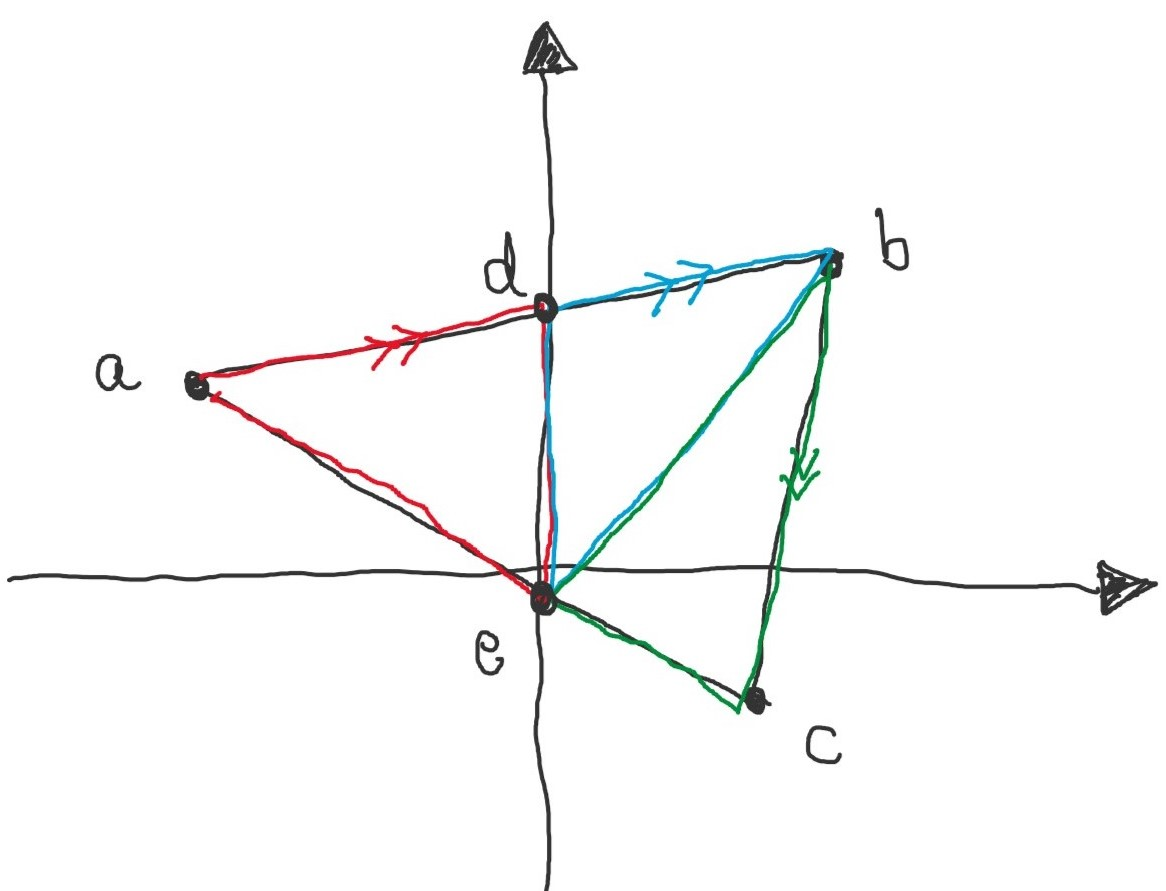
\includegraphics[height=3.5cm]{fkt_uebungen-5-abb.jpg}
	\end{center}
	Die Summe aller drei Wege ist wieder das originale Dreieck. Außerdem liegen alle \enquote{kleinen} Dreiecke nur in einer von beiden Halbebenen.
	Definiere
	\begin{equation*}
		\left.
		\begin{array}{ccccccc}
			\gamma_1 &\defeq& \sigma_{a,d} &\dot{+}& \sigma_{d,e} &\dot{+}& \sigma_{e,a} \\
			\gamma_2 &\defeq& \sigma_{d,b} &\dot{+}& \sigma_{b,e} &\dot{+}& \sigma_{e,d} \\
			\gamma_3 &\defeq& \sigma_{b,c} &\dot{+}& \sigma_{c,e} &\dot{+}& \sigma_{e,b} \\
		\end{array} 
		\right\} \follows
		\gamma = \gamma_1 \dot{+} \gamma_2 \dot{+} \gamma_3
	\end{equation*}
	wobei $\im(\gamma_1) \subseteq \quer{\CC^-}$ und $\im(\gamma_2), \im(\gamma_3) \subseteq \quer{\CC^+}$. Mit dem Hinweis gilt dann
	\begin{equation*}
		\int_{\gamma_i} f(z) \dz = 0 \quad \text{ für alle } i \in \menge{1,2,3}
	\end{equation*}
	Somit ist dann auch $\int_{\triangle(a,b,c)} f(z) \dz = 0$.
		
		
	\begin{task}
		Berechnen Sie das Integral
		\begin{equation*}
			\int_{-\infty}^\infty \frac{1}{1 + x^2} \dx
		\end{equation*}
		auf folgende Weise: Sei $R > 2$ und $\gamma_R$ der nebenstehende geschlossene Weg. Ermitteln Sie $\int_{\gamma_R} \frac{1}{1 + x^2} \dx$ mithilfe der Cauchyschen Integralformel und benutze $1 + z^2 = (z+\i) (z - \i)$. Dann Grenzübergang $R \to \infty$. 
		
		Hier darf folgende Variante des Zentrierungslemmas ohne Beweis verwendet werden: Ist $\abb{f}{\menge{z \in \CC : \Im(z) > -\frac{1}{2}} \setminus \menge{\i}}{\CC}$ holomorph, so gilt $\int_{\gamma_R} f(z) \dz = \int_{\abs{z-\i} = 1} f(z) \dz$.
		
		Berechnen Sie obiges Integral zur Probe auch mithilfe einer Stammfunktion von $x \mapsto \frac{1}{1 + x^2}$.
	\end{task}

	Parametrisiere den Weg $\gamma_R = \gamma_R^1 \dot{+} \gamma_R^2$ wie folgt: $\gamma_R^1 \defeq \id_{[-R,R]}$ und $\gamma_R^2(t) \defeq R*e^{\i t}$ für $t \in [0,\pi]$. Dann gilt 
	\begin{equation*}
		\abs{\int_{\gamma_R^2} \frac{1}{1+x^2} \dx} \le \pi R * \sup\menge{\abs{\frac{1}{1+x^2}} : \abs{x}=R, \Im(x) \ge 0} \le \frac{\pi R}{1 + R^2} \to 0 \tag{$R \to \infty$}
	\end{equation*}
	Mit der Cauchyschen Integralformel (CIF) erhält man dann
	\begin{align*}
		\lim_{R \to \infty} \int_{-R}^R \frac{1}{1 + x^2} \dx 
		&= \lim_{R \to \infty} \int_{\gamma_R^1} \frac{1}{1 + z^2} \dz \\
		&= \lim_{R \to \infty} \int_{\gamma_R} \frac{1}{1 + z^2} \dz \\
		&= \lim_{R \to \infty} \int_{\abs{z - \i} = 1} \frac{1}{(z- \i)(z + \i)} \dz \\
		&= \lim_{R \to \infty} 2\pi \i * \frac{1}{2\i}  \tag{CIF} \\
		&= \pi
	\end{align*}
	Zur Probe: Für $f(x) = \frac{1}{1 + x^2}$ ist eine Stammfunktion gegeben durch $F(x) = \arctan(x)$. Dann ist
	\begin{equation*}
		\int_{-\infty}^\infty f(x) \dx = \lim_{R \to \infty} \int_{-R}^R \frac{1}{1 + x^2} \dx = \lim_{R \to \infty} \brackets{\arctan(R) - \arctan(-R)} = \frac{\pi}{2} - \brackets{-\frac{\pi}{2}} = \pi
	\end{equation*}

	
	\begin{task}
		Sei $\abb{\gamma}{[0,1]}{\CC}$ ein geschlossener Weg. Zeigen Sie:
		\begin{equation*}
			\gamma \text{ nullhomotop} \follows \gamma \text{ nullhomolog}
		\end{equation*}		
	\end{task}

	Sei $\Omega \subseteq \CC$ offen und $\gamma$ nullhomotop in $\Omega$, d.h. homotop zu einem konstanten Weg $\abb{c}{[0,1]}{\CC}$. Dann gilt nach einer Bemerkung der Vorlesung für alle $\abb{f}{\Omega}{\CC}$ holomorph, dass $\int_\gamma f(z) \dz = \int_c f(z) \dz$. Da $c$ konstant ist, ist 
	\begin{equation*}
		\int_c f(z) \dz = \int_0^1 f(c(t)) * \underbrace{c'(t)}_{=0} \dt = 0
	\end{equation*}
	und somit also $\int_\gamma f(z) \dz = 0$ für alle holomorphen $\abb{f}{\Omega}{\CC}$. Nach Folgerung 9.4 ist dies äquivalent zur Nullhomologie von $\gamma$.
	
	
	\begin{task}
		Beweisen Sie das \textit{Schwarzsche Lemma}: Sei $\abb{f}{E}{E}$ eine holomorphe Abbildung der Einheitskreisscheibe $E$ in sich selbst mit $f(0) = 0$. Dann gilt $\abs{f'(0)} \le 1$ und $\abs{f(z)} \le \abs{z}$ für alle $z \in E$. Gibt es ein $z_0 \neq 0$ mit $\abs{f(z_0)} = \abs{z_0}$ oder gilt $\abs{f'(0)} = 1$, so ist $f$ eine Drehung mit $f(z) = e^{\i \theta} * z$ für ein $\theta \in \R$ und alle $z \in E$.
	\end{task}

	Wir definieren uns eine Funktion 
	\begin{equation*}
		\abb{g}{E}{\CC} \mit g(z) \defeq \begin{cases}
		\frac{f(z)}{z} & \text{falls } z \neq 0 \\
		f'(0)		   & \text{falls } z = 0
		\end{cases}
	\end{equation*}
	Damit ist $g$ stetig, denn
	\begin{equation*}
		g(0) = f'(0) = \lim_{z \to 0} \frac{f(z) - f(0)}{z - 0} = \lim_{z \to 0} \frac{f(z)}{z} = \lim_{\substack{z \to 0 \\ z \neq 0}} g(z)
	\end{equation*}
	Damit ist dann auch $g$ holomorph auf $E$. Für $r < 1$ gilt mit dem Maximumprinzip für $\abs{z} \le r$ 
	\begin{equation*}
		\abs{g(z)} \le \max_{\abs{z} = r} \abs{g(z)} = \frac{1}{r} * \max_{\abs{z} = r} \abs{f(z)} \le \frac{1}{r} \le 1
	\end{equation*}
	Somit ist also $\abs{g(z)} \le 1$ für alle $z \in E$, d.h. $\abs{\frac{f(z)}{z}} = \frac{\abs{f(z)}}{\abs{z}} \le 1 \follows \abs{f(z)} \le \abs{z}$ und $\abs{f'(0)} \le 1$.
	Ist $\abs{f(z_0)} = \abs{z_0}$ für ein $z_0 \neq 0$ oder $\abs{f'(0)} = 1$, so hat $\abs{g}$ im Inneren von $E$ ein lokales Maximum, was nach dem Maximumprinzip bedeutet, dass $g$ konstant ist, d.h. $g \equiv \lambda$ für ein $\lambda \in \CC$ mit $\abs{\lambda} = 1$ bzw. in Polardarstellung von $\lambda = e^{\i \theta}$ mit $\theta \in \R$ geschrieben als $f(z) = e^{\i \theta} * z$ für alle $z \in E$.
\end{exercisePage}
\begin{exercisePage}
	
	\begin{task}
		Bestimmen Sie die Potenzreihenentwicklung mit dem Mittelpunkt $z_0 \neq a$ für die Funktionen
		\begin{equation*}
			f_0(z) = \frac{1}{z-a} \qquad f_1(z) = \frac{1}{(z-a)^2} \qquad f_2(z) = \frac{1}{(z-a)^3}
		\end{equation*}
		Hinweis: Beachten Sie, dass $f_1 = -f_0*$ und $f_2 = -\frac{1}{2} f_1'$.
	\end{task}

	Unter Nutzung der geometrischen Reihe gilt
	\begin{equation*}
		\begin{aligned}
			f_0(z) = \frac{1}{z-a} = \frac{1}{(z-z_0) + z_0 - a} = \frac{1}{z_0 - a} * \frac{1}{1 + \frac{z-z_0}{z_0 - a}} 
			&= \frac{1}{z_0 - a} * \sum_{k=0}^\infty \frac{1}{(z_0 - a)^k} * (z-z_0)^k \\
			&=\sum_{k=0}^\infty \frac{1}{(z_0 - a)^{k+1}} * (z-z_0)^k
		\end{aligned}
	\end{equation*}
	d.h. wir haben eine Potenzreihe in $z_0$ mit Koeffizienten $a_k \defeq (z_0 - a)^{-(k+1)}$.
	Nutzen wir nun die Holomorphie und gliedweise Differenzierbarkeit infolge der Analytizität und erhalten
	\begin{equation*}
		f_1(z) = - f_0'(z) 
		= \sum_{k=0}^\infty \ableitung{z} \frac{1}{(z_0 - a)^{k+1}} * (z-z_0)^k 
		= \sum_{k=0}^\infty \frac{-(k+1)}{(z_0 - a)^{k+2}} * (z-z_0)^k
	\end{equation*}
	sowie
	\begin{equation*}
		f_2(z) = - \frac{1}{2} f_1'(z)
		= \sum_{k=0}^\infty \frac{1}{2} \ableitung{z} \frac{-(k+1)}{(z_0 - a)^{k+2}} * (z-z_0)^k
		= \sum_{k=0}^\infty \frac{(k+1)(k+2)}{2 (z_0 - a)^{k+3}} * (z-z_0)^k
	\end{equation*}
	
	\begin{task}
		Sei $\gamma \colon [0, 2\pi] \to \CC$, $\gamma(t) \defeq 2 e^{\i t}$. Berechnen Sie mithilfe der Cauchyschen Integralformeln für die Ableitungen das Integral $\int_\gamma f(z) \dz$ der folgenden Funktionen:
		\begin{enumerate}
			\item $f(z) = \frac{\cos(z)}{z^2}$
			\item $f(z) = \frac{z^3}{(z+\i)^3}$
			\item $f(z) = \frac{z * \cos(z)}{(z - \frac{\pi}{2})^2}$
			\item $f(z) = \frac{z * e^z}{(z-4)^3}$
		\end{enumerate} 
	\end{task}

	Sei $\Omega \subseteq \CC$ und $g \colon \Omega \to \CC$ holomorph auf $B_r(z_0)$. Weiter sei $z \notin \rand B_r(z_0)$. Dann gilt die Cauchysche Integralformel für die Ableitung von $g$ mit 
	\begin{equation*}
		g^{(k)}(z) = \frac{k!}{2 \pi \i} \int_{\abs{\xi - z_0} = r} \frac{g(\xi)}{(\xi - z)^{k+1}} \diffskip{\xi}
	\end{equation*}
	
	\begin{enumerate}[label=(zu \alph*), leftmargin=*]
		\item Betrachten wir $g(z) \defeq \cos(z)$ holomorph auf $\CC$ und $z = 0 \notin \rand B_2(0)$ sowie $z_0 = 0$. Dann gilt für die erste Ableitung ($k=1$)
		\begin{equation*}
			g'(0) = \frac{1!}{2 \pi \i} \int_{\abs{\xi} = 2} \frac{\cos(\xi)}{\xi^2} \diffskip{\xi}
		\end{equation*}
		und somit
		\begin{equation*}
			\int_\gamma f(z) \dz = 2 \pi \i * \cos'(0) = - 2 \pi \i \sin(0) = 0
		\end{equation*}
		
		\item Betrachte $g(z) \defeq z^3$ holomorph auf $\CC$ und $z = - \i \notin \rand B_2(0)$. Für die zweite Ableitung gilt diesmal 
		\begin{equation*}
			g''(-\i) = \frac{2}{2 \pi \i} \int_{\abs{\xi} = 2} \frac{\xi^3}{(\xi + \i)^3} \diffskip{\xi} 
		\end{equation*}
		Damit berechnen wir das Integral
		\begin{equation*}
			\int_\gamma f(z) \dz = \pi \i * g''(-\i) = \pi \i * 6 (-\i) = 6 \pi
		\end{equation*}
		
		\item Betrachte nun $g(z) \defeq z * \cos(z)$ holomorph auf $\CC$ und $z = \frac \pi 2 \notin B_2(0)$. Dann ist
		\begin{equation*}
			g'(\tfrac{\pi}{2}) = \frac{1}{2 \pi \i} \int_{\abs{\xi} = 2} \frac{\xi * \cos(\xi)}{(\xi - \tfrac{\pi}{2})^2} \diffskip{\xi}
		\end{equation*}
		d.h. für das Integral
		\begin{equation*}
			\int_\gamma f(z) \dz = 2 \pi \i * \left. \ableitung{z} z * \cos(z) \right\vert_{z = \tfrac{\pi}{2}} = 2 \pi \i \brackets{\cos\brackets{\tfrac{\pi}{2}} - \tfrac{\pi}{2} \sin\brackets{\tfrac{\pi}{2}}} = -\i \pi^2
		\end{equation*}
		
		\item Betrachte $g(z) \defeq z * e^z$ holomorph auf $\CC$ und $z = 4 \notin \rand B_2(0)$. Die zweite Ableitung ist
		\begin{equation*}
			g''(4) = \frac{2}{2 \pi \i} \int_{\abs{\xi} = 2} \frac{\xi * e^\xi}{(\xi - 4)^3} \diffskip{\xi} 
		\end{equation*}
		und damit
		\begin{equation*}
			\int_\gamma f(z) \dz = \pi \i * g''(4) = \pi \i \left. e^z (z+2) \right\vert_{z = 4} = 6 \pi \i * e^4
		\end{equation*}
	\end{enumerate}

	\begin{task}
		Entwickeln Sie die Funktion $\displaystyle f(z) = \frac{z}{(z-1)(z-2)}$ in Laurentreihen, die in folgenden Ringgebieten konvergieren:
		\begin{enumerate}
			\item $\abs{z} < 1$
			\item $1 < \abs{z} < 2$
			\item $\abs{z} > 2$
			\item $\abs{z-1} > 1$
		\end{enumerate}
	\end{task}

	\begin{task}
		Sei $\Omega \subseteq \Rn$ offen. Dann ist
		\begin{equation*}
			\Omega \text{ ist zusammenhängend} \equivalent \Omega \text{ ist wegzusammenhängend}
		\end{equation*}
	\end{task}

	\begin{equivalence}
		\rueckrichtung Diese Richtung haben wir bereits in der Vorlesung bewiesen.
		\hinrichtung Sei $\Omega \neq \emptyset$ (sonst klar). Dann existiert $z_0 \in \Omega$ --- betrachte 
		\begin{equation*}
			\mathcal{G}_{z_0} = \menge{z \in \Omega : \text{ex. Weg } \gamma \colon [0,1] \to \Omega \mit \gamma(0) = z_0 \und \gamma(1) = z}
		\end{equation*}
		Mit dem konstanten Weg ist stets $z_0 \in \Omega$, d.h. $\mathcal{G}_{z_0} \neq \emptyset$.
		
		Da $\Omega$ offen ist und $\mathcal{G}_{z_0} \subseteq \Omega$, existiert für alle $z \in \mathcal{G}_{z_0}$ ein $\epsilon > 0$ sodass $B_\epsilon(z) \subseteq \Omega$. Die $\epsilon$-Kugeln sind wegzusammenhängend, d.h. wir können den Weg von $z_0$ nach $z$ fortsetzen zu einem Weg von $z_0$ nach $\quer{z} \in B_\epsilon(z)$. Demnach ist $B_\epsilon(z) \subseteq \mathcal{G}_{z_0}$ für alle $z \in \mathcal{G}_{z_0}$. Somit ist $\mathcal{G}_{z_0}$ offen. 
		
		Betrachte $\mathcal{H}_{z_0} \defeq \Omega \setminus \mathcal{G}_{z_0}$. Gibt es $\omega \in \mathcal{H}_{z_0}$, dann gibt es auch $\epsilon > 0$ mit $B_\epsilon(\omega) \subseteq \Omega$. Angenommen es gibt nun ein $\quer{z} \in \mathcal{G}_{z_0} \cap B_\epsilon(\omega)$. Dann existiert ein fortgesetzter Weg von $z_0$ nach $\quer{z}$, was heißen würde, dass $\omega \in \mathcal{G}_{z_0}$ im Widerspruch zur Annahme. Damit ist $B_\epsilon(\omega) \subseteq \mathcal{H}_{z_0}$. 
		
		Damit ist $\Omega = \mathcal{G}_{z_0} \cupdot \mathcal{H}_{z_0}$. Jedoch ist $\mathcal{G}_{z_0} \neq \emptyset$, d.h. es muss $\mathbb{H}_{z_0} = \emptyset$ und $\Omega = \mathcal{G}_{z_0}$ gelten. Damit ist $\Omega$ wegzusammenhängend.
	\end{equivalence}

	\begin{task}
		Man beweise, dass es eindeutig bestimmte ganze Funktionen $J_n$ gibt, sodass für alle $(z,\zeta) \in \CC \times (\CC \setminus \menge{0})$ die Gleichung
		\begin{equation*}
			\exp\brackets{\frac{z}{2} \brackets{\zeta - \frac{1}{\zeta}}} = \sum_{n = -\infty}^\infty J_n(z) * \zeta^n
		\end{equation*}
		gilt.
	\end{task}
\end{exercisePage}

\end{document}